% !TEX root = ../main.tex
\renewcommand{\localPath}{chap3}

\chapter{Modèle hybride linéarisé dans~le~cas~$1dz-3dv$}
\label{chap3}

Ce chapitre est la seconde partie d'une étude du modèle hybride linéarisé~\eqref{eq:0:vmhl:1}-\eqref{eq:0:vmhl:4} dans le cadre restreint $1dz-3dv$. Il s'agit d'utiliser les concepts du chapitre précédent et de les étendre au cas multi-dimensionnel en vitesse pour prendre en compte les effets du champ magnétique. La manipulation de variables vectorielles impose une généralisation du cadre scalaire étudié dans le chapitre~\ref{chap1}. Ce travail collaboratif avec Anaïs Crestetto\footnote{Université de Nantes, laboratoire de Mathématiques Jean Leray}, Nicolas Crouseilles\footnote{Univ Rennes, Inria Bretagne Atlantique (MINGuS) \& ENS Rennes} et Yingzhe Li\footnote{Max Planck Institute, Institut Für Plasmaphysik, Germany} a mené à un article \emph{Comparison of high-order Eulerian methods for electron hybrid model} soumis dans \emph{Journal of Computational Physics} en 2021.

%% section 1
% !TEX root = ../chap3.tex

\section{Introduction}

L'objectif de ce chapitre est d'étendre les stratégies développées pour la résolution d'un modèle hybride linéarisé, présentées dans le chapitre~\ref{chap2}, au cas $1dz-3dv$ permettant de prendre en compte, entre autre, les effets du champ magnétique sur la dynamtique des particules. Nous étudierons dans ce chapitre un modèle hybride, ce qui suppose que la distribution de particules est composée de deux populations, une première ayant une vitesse thermique faible, et considérée comme \emph{froide}, dont on approximera la dynamique comme celle d'un fluide ; une seconde population ayant une vitesse thermique plus élevée, considérée comme \emph{chaude}, mais contrairement au chapitre~\ref{chap2}, celle-ci n'a pas besoin d'être distribuée selon une bi-maxwellienne. Ce type de modèle peut être utilisé pour modéliser des particules d'un plasma dans un tokamak, ou des particules du vent solaire interagissant avec la magnétosphère terrestre. Dans ces contextes les particules se déplacent de manière hélicoïdale selon les lignes du champ extérieur $\vb{B}_0 = (0,0,B_0)^\top$, et seul le déplacement dans cette direction sera étudié ici, ce qui explique le nom de la seule variable d'espace considérée : $z$. Pour le déplacement hélicoïdale complet \Josselin{il faudrait ajouter ici une référence que je n'ai pas car je ne connais pas trop ces modèles, de mémoire c'est ce que faisait Xiaofei}.

La prise en compte des effets du champ magnétique dans le modèle nous mène à considérer un système à 7 inconnues $(j_{c,x},j_{c,y},B_x,B_y,E_x,E_y,f_h)$, ce qui induit un coût de calcul bien plus important avec les méthodes eulériennes que nous étudions. Pour diminuer ce coût de calcul nous souhaitons diminuer le nombre d'itérations tout en assurant la stabilité des méthodes considérées ; cela se fait en augmentant le pas de temps $\Delta t$ et en estimant les contraintes de stabilité. L'utilisation de méthodes d'ordre élevés en temps, en espace et en vitesse, permet de réduire l'erreur, capturer la dynamique non-linéaire du système, avec peu de points de discrétisation.

Nous souhaitons dans ce chapitre comparer deux méthodes d'ordre élevé en temps et dans l'espace des phrases, sur un cas à 4 dimensions, plus proches d'applications physiques, il s'agit d'une généralisation des deux stratégies développées dans le chapitre~\ref{chap2}, une méthode de \emph{splitting} et une méthode de Lawson. La contrainte du nombre de dimensions ne permet pas de raffiner le maillage\footnote{Pour une discrétisation de $128$ points par direction, la grille contient $128^4$ points, soit, représentées avec des réels à virgule flottante à double précision (64 bits), un espace mémoire de 2Go pour la seule variable $f_h$ ; une méthode de Lawson d'ordre 4 nécessite la sauvegarde des étages intermédiaires, donc $4\times 2\textrm{Go}$ minimum. L'utilisation de transformées de Fourier impose de travailler avec des nombres complexes, ce qui nécessite de doubler l'utilisation mémoire pour la même précision.}, ce qui ne permet pas l'accès à une solution de référence, nous devrons nous contenter de regarder les invariants (comme l'énergie totale), et de comparer les résultats aux taux d'instabilités fournis par les relations de dispersion.

Pour résoudre les problèmes que pose ce problème nous présenterons tout d'abord le modèle hybride $1dz-3dv$, puis nous détaillerons les schémas numériques que nous considérons. La méthode de \emph{splitting} hamiltonien contient 7 étapes, rendant de fait l'ordre élevé (méthode de Suzuki) trop coûteux pour approfondir son étude, nous nous concentrerons donc sur des méthodes de \emph{splitting} d'ordre plus faible. Pour la méthode de Lawson, il est envisageable d'effectuer un filtrage du terme induit pas le champ magnétique externe $\vb{B}_0$, permettant d'augmenter le pas de temps stabilisant la méthode. La partie linéaire du système introduit une matrice dont il n'est pas possible de calculer exactement son exponentielle, pourtant nécessaire pour la mise en œuvre d'une méthode de Lawson perforante. Nous étudierons un premier cas où nous ne profitons pas pleinement de toute la partie linéaire du système, introduisant ainsi une condition de stabilité ; puis nous proposerons une méthode permettant, à l'aide de méthodes approchées comme la troncature de la série de Taylor ou les approximants de Padé, de calculer une approximation de l'exponentielle de toute la partie linéaire, permettant ainsi de se soustraire à une condition de stabilité. \Josselin{Mettre les références vers les sections.}

%% section 2
% !TEX root = ../chap3.tex

\section{Présentation du modèle}

\begin{align}
  \label{eq:VHM:jx}
  &\pdv{j_{c,x}}{t} = \Omega_{pe}^2 { E}_x - { j}_{c,y}B_0,\\
  \label{eq:VHM:jy}
  &\pdv{j_{c,y}}{t} = \Omega_{pe}^2 { E}_y + { j}_{c,x}B_0,\\
  \label{eq:VHM:Bx}
  &\pdv{B_{x  }}{t} = \partial_z E_y,\\
  \label{eq:VHM:By}
  &\pdv{B_{y  }}{t} = -\partial_z E_x,\\
  \label{eq:VHM:Ex}
  &\pdv{E_{x  }}{t} =-\partial_z B_y - {j}_{c,x} + \int v_x f_h \dd{\vb{v}},\\
  \label{eq:VHM:Ey}
  &\pdv{E_{y  }}{t} =\partial_z B_x - {j}_{c,y} + \int v_y f_h \dd{\vb{v}}, \\
  \label{eq:VHM:fh}
  &\pdv{f_{h  }}{t} +  v_z\partial_z f_h - \left(E_x + v_y B_0 - v_zB_y\right)\partial_{v_x} f_h\\
  &\hspace{2cm}- \left(E_y - v_x B_0 + v_z B_x\right)\partial_{v_y} f_h- \left(v_x B_y- v_y B_x\right)\partial_{v_z} f_h = 0.\nonumber
\end{align}
Cela nous permet de définir l'hamiltonien :
\begin{equation}
  \mathcal{H} = {}
      \underbrace{\frac{1}{2}\int_{\mathbb{R}}(E_x^2+E_y^2) \dd{z}}_{\mathcal{H}_E}
    + \underbrace{\frac{1}{2}\int_{\mathbb{R}}(B_x^2+B_y^2) \dd{z}}_{\mathcal{H}_B}
    + \underbrace{\frac{1}{2}\int_{\mathbb{R}}\frac{1}{\Omega_{pe}^2}(j_{c,x}^2+j_{c,y}^2) \dd{z}}_{\mathcal{H}_{j_c}}
    + \underbrace{\frac{1}{2}\int_{\mathbb{R}}\int_{\mathbb{R}^2}|\vb{v}|^2 f_h \dd{\vb{v}}\dd{z}}_{\mathcal{H}_{f_h}}
  \label{eq:ham1dz3dv}
\end{equation}

On définit le crouchet suivant, définit pour deux fonctionnelles $\mathcal{F}$ et $\mathcal{G}$ :
\begin{equation}
  \begin{aligned}
    \{ \mathcal{F},\mathcal{G} \}[ j_{c,x}, j_{c,y}, B_x, B_y, E_x, E_y, f_h] &=
                       \int_{\mathbb{R}}\int_{\mathbb{R}^3} f_h \left( \partial_z\fdv{\mathcal{F}}{f_h}\partial_{v_z}\fdv{\mathcal{G}}{f_h} - \partial_{v_z}\fdv{\mathcal{F}}{f_h}\partial_z\fdv{\mathcal{G}}{f_h} \right) \dd{\vb{v}}\dd{z} \\
      &\hspace{-4cm} + \int_{\mathbb{R}}\int_{\mathbb{R}^3} f_h \left(
            \partial_{v_x}\fdv{\mathcal{F}}{f_h}\fdv{\mathcal{G}}{E_x} + \partial_{v_y}\fdv{\mathcal{F}}{f_h}\fdv{\mathcal{G}}{E_y}
          - \partial_{v_x}\fdv{\mathcal{G}}{f_h}\fdv{\mathcal{F}}{E_x} - \partial_{v_y}\fdv{\mathcal{G}}{f_h}\fdv{\mathcal{F}}{E_y}
          \right) \dd{\vb{v}}\dd{z} \\
      &\hspace{-4cm} + \int_{\mathbb{R}}\int_{\mathbb{R}^3} f_h(\vb{B}+\vb{B}_0)\cdot\left( \nabla_{\vb{v}}\fdv{\mathcal{F}}{f_h}\times\nabla_{\vb{v}}\fdv{\mathcal{G}}{f_h} \right) \dd{\vb{v}}\dd{z} \\
      &\hspace{-4cm} + \int_{\mathbb{R}} \left(
          - \partial_z\fdv{\mathcal{F}}{E_y}\fdv{\mathcal{G}}{B_x} + \partial_z\fdv{\mathcal{F}}{E_x}\fdv{\mathcal{G}}{B_y}
          + \partial_z\fdv{\mathcal{G}}{E_y}\fdv{\mathcal{F}}{B_x} - \partial_z\fdv{\mathcal{G}}{E_x}\fdv{\mathcal{F}}{B_y}
          \right) \dd{z} \\
      &\hspace{-4cm} + \int_{\mathbb{R}} \Omega_{pe}^2 \left(
            \fdv{\mathcal{F}}{j_{c,x}}\fdv{\mathcal{G}}{E_x} + \fdv{\mathcal{F}}{j_{c,y}}\fdv{\mathcal{G}}{E_y}
          - \fdv{\mathcal{G}}{j_{c,x}}\fdv{\mathcal{F}}{E_x} - \fdv{\mathcal{G}}{j_{c,y}}\fdv{\mathcal{F}}{E_y}
          \right) \dd{z} \\
      &\hspace{-4cm} + \int_{\mathbb{R}} \Omega_{pe}^2B_0 \left(
            \fdv{\mathcal{F}}{j_{c,x}}\fdv{\mathcal{G}}{j_{c,y}}
          - \fdv{\mathcal{F}}{j_{c,y}}\fdv{\mathcal{G}}{j_{c,x}}
          \right) \dd{z}.
  \end{aligned}
  \label{bracket}
\end{equation}
Cela nous permet de réécrire le système~\eqref{eq:VHM:jx}-\eqref{eq:VHM:fh} comme 
$$
  \partial_t U = \{ U,\mathcal{H} \}
$$
où $U(t,z,\vb{v}) = ( j_{c,\perp}(t,z) , B_\perp(t,z) , E_\perp(t,z) , f)h(t,z,\vb{v}) )^\top$ où $\mathcal{H}$ est donné par~\eqref{eq:ham1dz3dv} et $j_{c,\perp}=(j_{c,x},j_{c,y})^\top$, $B_{\perp}=(B_{x},B_{y})^\top$ et $E_{\perp}=(E_{x},E_{y})^\top$. Par la suite, nous utiliserons également les notations $v_\perp = (v_x,v_y)^\top\in\mathbb{R}^2$ ainsi que $\vb{v} = (v_\perp,v_z)^\top\in\mathbb{R}^3$ et nous définissions la matrice symplectique 
$$
  J = \begin{pmatrix}
     0 & 1 \\
    -1 & 0
  \end{pmatrix}.
$$

%% section 3
% !TEX root = ../../main.tex

\section{Méthodes de résolution numérique en temps}
%%%%%%%%%%%%%%%%%%%%%%%%%%%%%%%%%%%%%%%%%%%%%%%%%%%%%%%%%%%%%%%%%%%%%%

Dans cette section nous allons présenter les principales méthodes utilisées pour résoudre numériquement des équations dites cinétiques en temps, et plus spécifiquement le système~\eqref{eq:0:vmhl:1}-\eqref{eq:0:vmhl:4}. Une fois discrétisé en $(\vb{x},\vb{v})$, les différents systèmes que nous regardons peuvent se réduire au modèle abstrait suivant :
\begin{equation}
  \dot{u} = L(t,u) + N(t,u),\quad u(0)=u_0
  \label{eq:0:dtu}
\end{equation}
d'inconnue $u\in\mathbb{R}^n$ et où $L$ et $N$ sont des fonctions $(t,u)\in\mathbb{R}_+\times\mathbb{R}^n\mapsto\mathbb{R}^n$, $n\in\mathbb{N}$ est le nombre de dimensions, ou d'inconnues du problème. C'est sur cette équation~\eqref{eq:0:dtu} que nous allons présenter les différentes méthodes d'intégration en temps utilisées ici.

% --------------------------------------------------------------------
\subsection{Méthode de \emph{splitting} hamiltonien}
% --------------------------------------------------------------------

Les méthodes de \emph{splitting} sont classiquement utilisées dans la résolution d'équations cinétiques (\cite{Morrison:2017,Grandgirard:2006,Tronci:2010,Tronci:2014}), elles consistent à diviser l'équation à résoudre en plusieurs parties. La construction de ces méthodes en temps se fait par concaténation des différentes étapes en formant des palindromes.

Une méthode de \emph{splitting} consiste à résoudre les deux équations suivantes successivement :
\begin{eqnarray}
    \dot{u} = L(t,u)\label{eq:0:split:1}\\
    \dot{u} = N(t,u)\label{eq:0:split:2}
\end{eqnarray}
La solution de l'équation~\eqref{eq:0:dtu} au temps $t$ est $\varphi_t(u_0)$, et sera approchée par une composition de $\varphi_t^{[L]}(u_0)$ et $\varphi_t^{[N]}(u_0)$, respectivement solutions de~\eqref{eq:0:split:1} et~\eqref{eq:0:split:2}. Ainsi la méthode de Lie, \emph{splitting} d'ordre 1, consiste à approcher $\varphi_t(u_0)$ par $\varphi_t(u_0)\approx \varphi_t^{[L]} \circ \varphi_t^{[N]}(u_0)$. Si la résolution de chaque sous-système $\varphi_t^{[L]}$ et $\varphi_t^{[N]}$ est exacte, la seule erreur en temps provient du \emph{splitting}.

La résolution de chaque sous-système peut se faire sur des intervalles de temps différents (que nous noterons en indice), ainsi la méthode de Strang~\cite{Strang:1968}, \emph{splitting} d'ordre 2, s'écrit comme :
$$
  u(t) = S_{t}(u_0) = \varphi^{[L]}_{t/2}\circ\varphi^{[N]}_{t}\circ\varphi^{[L]}_{t/2}(u_0)
$$

Lorsque l'équation met en jeu plusieurs termes, comme c'est le cas pour le système~\eqref{eq:0:vmhl:1}-\eqref{eq:0:vmhl:4}, il est difficile de savoir comment choisir $L$ et $N$. L'hamiltonien du système permet de suggérer une décomposition intéressante, et de construire des méthodes appelées \emph{splitting} hamiltonien~\cite{Crouseilles:2015,Casas:2017,Bernier:2020,Li:2019}.


\subsection{Méthode de type Runge-Kutta}
% --------------------------------------------------------------------

Les méthodes de type Runge-Kutta sont des méthodes d'approximation de solutions d'équations différentielles, développées dès 1901. Elles peuvent être vues comme une extension, à des ordres supérieurs, de la méthode d'Euler. Nous utiliserons ce type de méthodes pour résoudre la discrétisation en temps. Nous allons présenter ce type de méthode sur l'équation :
$$
  \dot{u} = N(t,u),\qquad u(0)=u_0
$$
où $u\in\mathbb{R}^n$, et $N:(t,u)\in\mathbb{R}_+\times\mathbb{R}^n\mapsto N(t,u)\in\mathbb{R}^n$ une fonction agissant sur $u$ et pouvant dépendre du temps $t$. Il s'agit d'un cas particulier de l'équation~\eqref{eq:0:dtu} où $L$ est la fonction nulle. Nous résumerons les méthodes par leur tableau de Butcher\cite{Butcher:2008}, qui se représentent sous la forme :
\begin{equation}  
  \begin{array}{c|c}
    \begin{matrix}
      c_1 \\
      \vdots \\
      c_s
    \end{matrix}
    &
    \begin{matrix}
      a_{11} & \cdots & a_{1s} \\
      \vdots & \ddots & \vdots \\
      a_{s1} & \cdots & a_{ss}
    \end{matrix} \\
    \hline
     & \begin{matrix} b_1 & \cdots & b_s \end{matrix} \\
  \end{array}
  \label{eq:0:butcher}
\end{equation}
et qui se lit :
$$
  \begin{aligned}
    u^{(i)} &= u^n + \Delta t \sum_{j=1}^s a_{ij} N(t^n+c_j\Delta t,u^{(j)}) \\
    u^{n+1} &= u^n + \Delta t \sum_{i=1}^s b_i N(t^n+c_i\Delta t, u^{(i)}),
  \end{aligned}
$$
où $u^n\approx u(t^n)$ avec $t^n=n\Delta t$, et où $\Delta t$ est le pas de temps.

Nous n’étudierons, pour des raisons de performances numériques, que des méthodes dites explicites, c'est-à-dire que chaque étage ne nécessite que les étages précédents pour être calculé. Dans ce cas, la matrice $(a_{ij})_{i,j}$ est triangulaire strictement inférieure. Dans le cadre de méthode explicite, il est possible de convertir la méthode, comme la méthode RK(3,3) de Shu-Osher, pour n'avoir qu'une seule évaluation de la fonction non linéaire $N$ par étage de la méthode.

Un intérêt des méthodes de type Runge-Kutta explicite est la montée en ordre. En effet celle-ci peut se faire de manière presque linéaire par rapport au nombre d'étages. À l'inverse, ces méthodes ne préservent pas l'énergie du système qu'elles résolvent, la montée en ordre est donc une nécessité pour réduire l'erreur et garantir la validité des résultats. Un autre inconvénient de ce type de résolution est l'introduction de condition de stabilité, que nous détaillerons un peu plus dans le cadre du chapitre~\ref{chap1}.

Nous bénéficions de la large littérature sur le sujet des méthodes de type Runge-Kutta, l'étude de stabilité ou de convergence (voir~\cite{Shu:2001,Butcher:2008,Gottlieb:2011,Baldauf:2008,Spiteri:2002}), ainsi que des améliorations dans des contextes spécifiques ; telles que les méthodes de Dormand-Prince permettant des stratégies de pas de temps adaptatifs (voir~\cite{Dormand:1978,Dormand:1980,,Gustafsson:1988,,Gustafsson:1994,Balac:2013,Balac:2014}), ou les méthodes de Lawson qui profitent de la structure linéaire de l'équation (voir~\cite{Lawson:1967,Isherwood:2018,Hochbruck:2020}).

\subsubsection{Méthode de Lawson}
% --------------------------------------------------------------------
\label{ssec:0:lawson}

Les méthodes de Lawson sont une optimisation des méthodes de type Runge-Kutta à des équations ayant une partie linéaire que l'on écrit comme suit :
$$
  \dot{u}(t) = Lu(t) + N(t,u)
$$
il s'agit du cas particulier de l'équation~\eqref{eq:0:dtu} où $L$ est une matrice ou un opérateur linéaire agissant sur $u$. Le principe de la méthode de Lawson est d'utiliser une formule de Duhamel sur $u$ pour résoudre exactement le terme linéaire. Ceci permet de se soustraire d'une condition de stabilité provenant du terme linéaire, et réduire l'erreur en résolvant exactement le plus de termes possibles.

Nous effectuons une formule de Duhamel en notant $v = e^{-tL}u$, ce qui nous permet de calculer :
$$
  \dot{v}(t) = -Le^{-tL}u(t) + e^{-tL}\dot{u}(t)
$$
d'où :
$$
  \dot{v}(t) = -Le^{-tL}u(t) + e^{-tL}Lu(t) + e^{-tL}N(t,u).
$$
On peut maintenant écrire l'équation sur $v$ que nous souhaitons résoudre avec une méthode de type Runge-Kutta :
$$
  \dot{v} = \tilde{N}(t,v)
$$
avec $\tilde{N}:(t,v)\in\mathbb{R}_+\times\mathbb{R}^n\mapsto e^{-tL}N(t,e^{tL}v)\in\mathbb{R}^n$. La méthode de Lawson consiste à réécrire la méthode Runge-Kutta sur $v$ en la variable $u$, où la partie linéaire est résolue exactement. La méthode de Lawson, induite par une méthode Runge-Kutta explicite décrite par le tableau de Butcher~\eqref{eq:0:butcher}, s'écrit alors :
$$
  \begin{aligned}
    u^{(i)} &= e^{c_i\Delta t L}u^n + \Delta t \sum_{j=1}^{i-1} a_{ij}e^{-(c_j-c_i)\Delta t L}N(t^n+c_j\Delta t,u^{(j)}) \\
    u^{n+1} &= e^{\Delta t L}u^n + \Delta t \sum_{i=1}^{s} b_i e^{(1-c_i)\Delta tL} N(t^n+c_i\Delta t,u^{(i)})
  \end{aligned}
$$

Le cadre théorique pour l'étude de convergence de schémas a été proposé dans~\cite{Hochbruck:2010,Hochbruck:2020}. Comme pour une méthode Runge-Kutta classique, il est possible d'appliquer la même méthode d'optimisation de Shu-Osher pour n'avoir qu'une seule évaluation de la fonction non-linéaire $N$ par étage dans le cadre d'une méthode explicite.


\section{Méthodes de résolution numérique en espace}
%%%%%%%%%%%%%%%%%%%%%%%%%%%%%%%%%%%%%%%%%%%%%%%%%%%%%%%%%%%%%%%%%%%%%%

Nous présentons dans cette section les méthodes numériques permettant de discrétiser en espace ($\vb{x}$ ou $\vb{v}$) que nous allons utiliser pour résoudre numériquement le système~\eqref{eq:0:vmhl:1}-\eqref{eq:0:vmhl:4}.

% --------------------------------------------------------------------
\subsection{Méthode WENO}
% --------------------------------------------------------------------

La méthode WENO, pour \emph{Weighted Essentially Non-Oscillatory}, est une méthode volumes finis ou différences finies, dont l'écriture classique est d'ordre 5. Il s'agit d'une méthode \emph{upwind}, d'ordre élevé, combinée à des poids non-linéaires permettant de réduire les oscillations par de la baisse d'ordre et de la diffusion numérique. La méthode d'ordre 5 est présentée dans \cite{Liu:1994,Jiang:1996,Shu:1999,Shu:2003}. Nous la présentons ici pour une équation de transport de la forme :
\begin{equation}
  \partial_t u + \partial_x f(u) = 0,\qquad u(t=0,x) = u_0(x)
  \label{eq:0:dtudxfu}
\end{equation}
avec $u(t,x)$ la fonction inconnue dépendant du temps $t\geq 0$ et de l'espace $x\in\Omega$ (supposé ici périodique par commodité), et $f:u\mapsto f(u)$ une fonction agissant sur $u$. On définit une discrétisation de l'espace $x_i = i\Delta x + x_0$, $i=0,\dots,N_x$, avec $\Delta x>0$ le pas d'espace. La méthode WENO se présente comme suit :
$$
  \partial_t u_j(t) + \frac{1}{\Delta x}\left( \hat{f}_{j+\frac{1}{2}} - \hat{f}_{j-\frac{1}{2}} \right) = 0,
$$
où $u_j(t)\approx u(t,x_j)$, $j=0,\dots,N$, et où $\hat{f}_{j+\frac{1}{2}} = \hat{f}(u_{j-2},\dots,u_{j+2})$ est le flux numérique, ici présenté pour WENO5, avec $(u_{j-2},\dots,u_{j+2})$ le \emph{stencil} de la méthode, c'est-à-dire le voisinage de points nécessaire pour calculer une approximation de la dérivée en espace. Comme pour une méthode \emph{upwind}, il est nécessaire de distinguer le flux en deux parties, positive et négative :
$$
  f(u) = f^+(u) + f^-(u).
$$
Pour cela il est possible d'utiliser le flux de Lax-Friedrichs (voir~\cite{Shu:1997}). Dans les cas qui nous intéressent, $f:u\mapsto au$ est une fonction linéaire, il est donc simplement nécessaire de connaître le signe de la vitesse d'advection $a$, on note alors $a^+ = \max(a,0)$ et $a^-=\min(a,0)$ et on a $f^\pm_j=f^\pm(u_j)=a^\pm u_j$.

\begin{figure}[h]
  \centering
  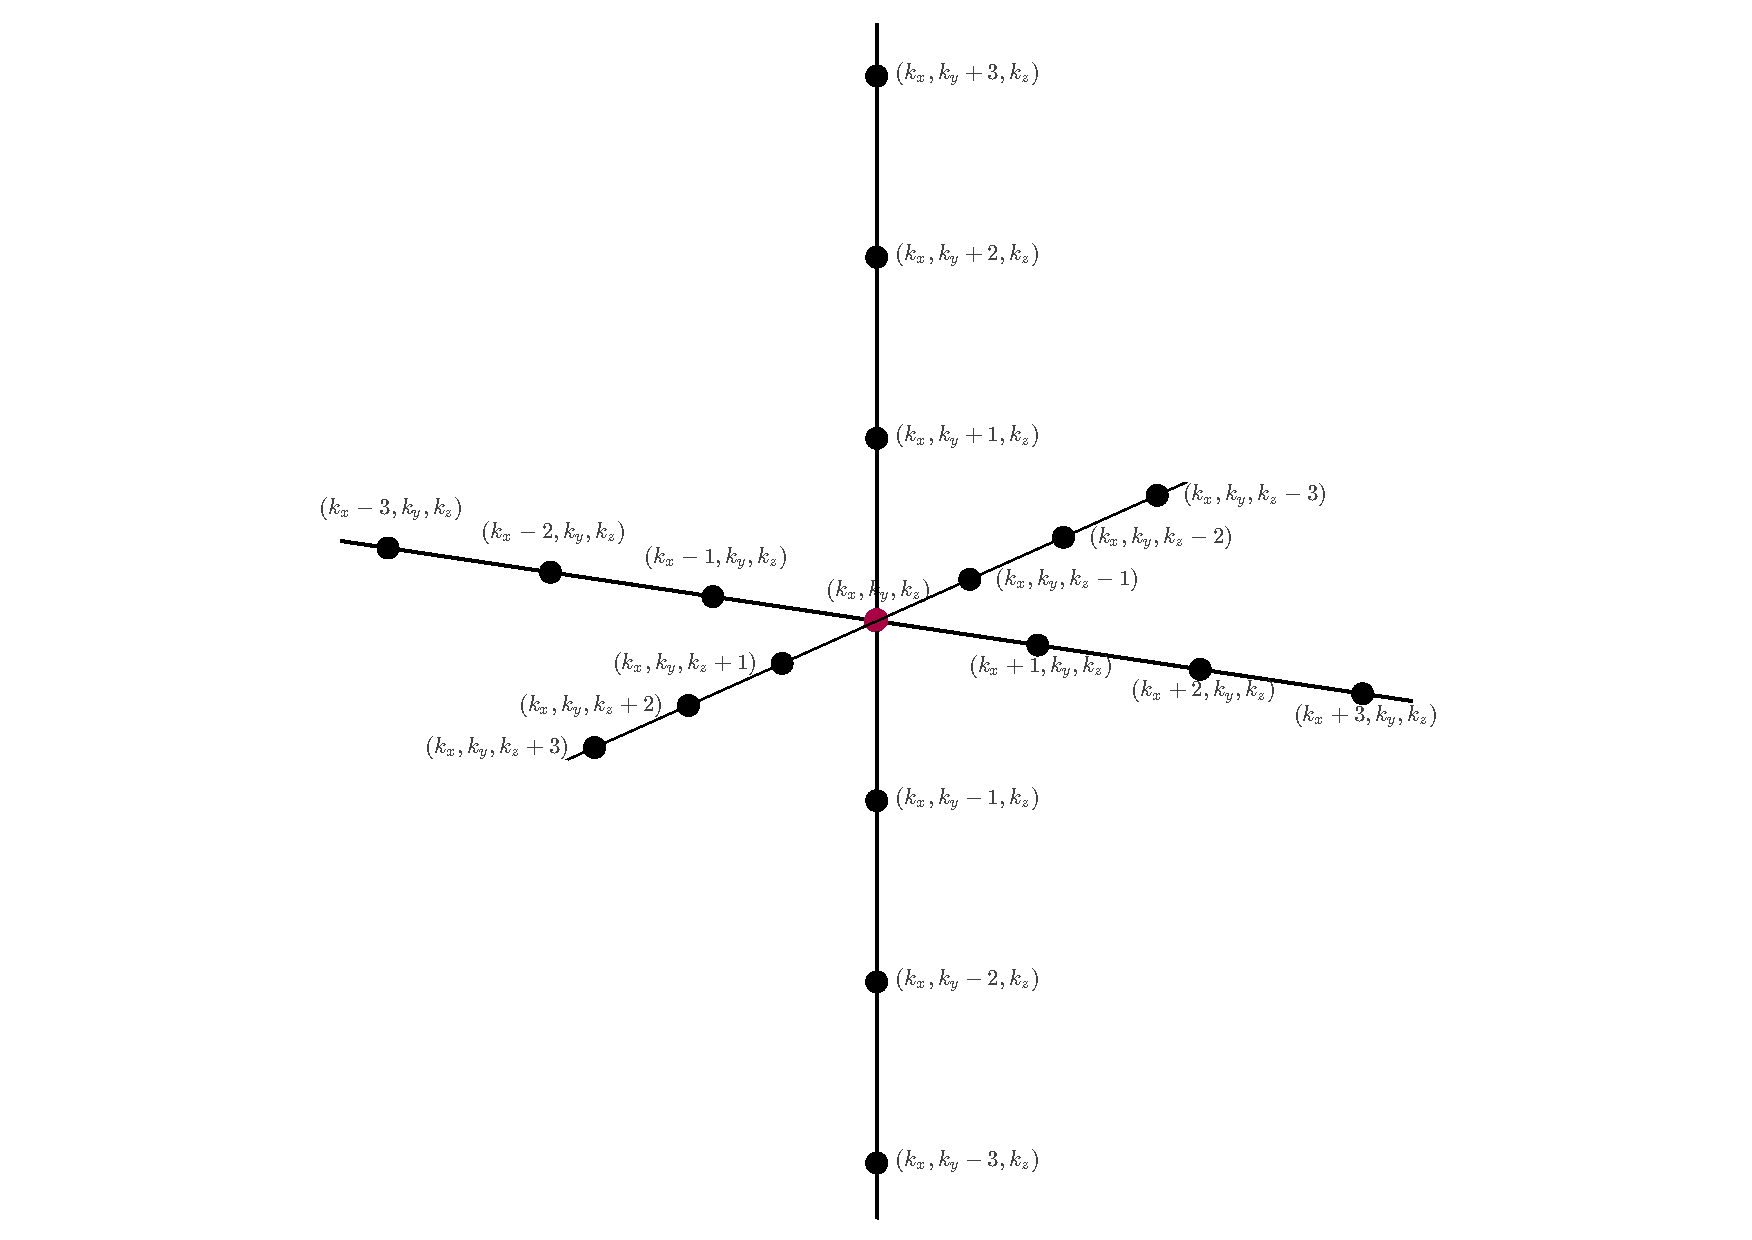
\includegraphics[width=0.9\textwidth]{\localPath/figures/stencil.pdf}
  \caption{Présentation des \emph{stencils} utilisés par la méthode WENO5 pour calculer le flux numérique.}
  \label{fig:intro:stencil}
\end{figure}

La méthode WENO5 consiste en 3 interpolations, sur 3 \emph{stencils} différents, comme l'illustre la figure~\ref{fig:intro:stencil}, pondérées par des poids non-linéaires issus des approximations des dérivées successives de $f$. L'écriture des poids s'effectue comme suit dans le cas $f^-=0$ :
$$
  \begin{aligned}
    \beta_0 &= \frac{13}{12}( \underbrace{f^+_{j-2} - 2f^+_{j-1} + f^+_{j}}_{\Delta x^2(f''_{j} + \mathcal{O}(\Delta x))})^2   + \frac{1}{4}( \underbrace{  f^+_{j-2} - 4f^+_{j-1} + 3f^+_{j}  }_{ 2\Delta x ( f'_{j} + \mathcal{O}(\Delta x^2))})^2 \\
    \beta_1 &= \frac{13}{12}( \underbrace{f^+_{j-1} - 2f^+_{j}   + f^+_{j+1}}_{\Delta x^2(f''_{j} + \mathcal{O}(\Delta x^2))} )^2 + \frac{1}{4}( \underbrace{  f^+_{j-1} -               f^+_{j+1}}_{ 2\Delta x   f'_{j} + \mathcal{O}(\Delta x^2))})^2 \\
    \beta_2 &= \frac{13}{12}( \underbrace{f^+_{j}   - 2f^+_{j+1} + f^+_{j+2}}_{\Delta x^2(f''_{j} + \mathcal{O}(\Delta x))} )^2   + \frac{1}{4}( \underbrace{ 3f^+_{j}   - 4f^+_{j+1} +  f^+_{j+2}}_{-2\Delta x ( f'_{j} + \mathcal{O}(\Delta x^2))})^2 \\
  \end{aligned}
$$
où les coefficients $\beta_0$ sont appelés indicateurs de continuité (\emph{indicators of smoothness}). Ce qui nous permet de calculer les poids définis par :
$$
  \alpha_i = \frac{\gamma_i}{(\varepsilon + \beta_i)^2},\quad i=0,1,2
$$
où $\varepsilon$ est un paramètre numérique pour assurer la non nullité du dénominateur, il sera pris à $10^{-6}$ ; et avec $\gamma_0=\frac{1}{10}$, $\gamma_1=\frac{6}{10}$ et $\gamma_2=\frac{3}{10}$. La normalisation des poids s'effectue comme suit :
$$
  w_i = \frac{\alpha_i}{\sum_m \alpha_m},\quad i=0,1,2
$$
Nous pouvons ensuite calculer les flux numériques pour WENO5 \cite{Shu:2003}, donnés par :
$$
  \begin{aligned}
    \hat{f}_{j+\frac{1}{2}}^+   =\ & w_0\left(  \frac{2}{6}f^+_{j-2} - \frac{7}{6}f^+_{j-1} + \frac{11}{6}f^+_{j}   \right)
                                +    w_1\left( -\frac{1}{6}f^+_{j-1} + \frac{5}{6}f^+_{j}   +  \frac{2}{6}f^+_{j+1} \right) \\
                                +  & w_2\left(  \frac{2}{6}f^+_{j}   + \frac{5}{6}f^+_{j+1} -  \frac{1}{6}f^+_{j+2} \right).
  \end{aligned}
$$
La méthode WENO5 prend la forme finale :
$$
  \partial_xf(x_j) \approx \frac{1}{\Delta x}\left[ \left(\hat{f}_{j+\frac{1}{2}}^+ - \hat{f}_{j-\frac{1}{2}}^+ \right) + \left(\hat{f}_{j+\frac{1}{2}}^- - \hat{f}_{j-\frac{1}{2}}^- \right) \right].
$$

Il existe des variantes de la méthode WENO5, permettant de réduire la perte d'ordre à l'approche d'un choc, à savoir WENO-M (\cite{Henrick:2005}) ou WENO-Z (\cite{Borges:2008}). Ces variations se font sur le calcul des poids non-linéaires. Ainsi la méthode WENO-M utilise une fonction de \emph{mappage} pour équilibrer les poids et est définie par :
$$
  \begin{aligned}
    \alpha_i    &= \frac{\gamma_i}{(\epsilon + \beta_i)^2} \\
    \tilde{w}_i &= \frac{\alpha_i}{\sum_k \alpha_k} \\
    g_i         &= w_i\left( \frac{\gamma_i + \gamma_i^2 - 3w_i\gamma_i + w_i^2}{\gamma_i^2 + w_i(1-2\gamma_i)} \right) \\
    w_i         &= \frac{g_i}{\sum_k g_k}
  \end{aligned}
$$
avec le paramètre $\epsilon = 10^{-4}$. La méthode WENO-Z est quant à elle définie par :
$$
  \begin{aligned}
    \alpha_i &= \gamma_i\left( 1+ \frac{\tau_5}{\epsilon + \beta_i} \right) \\
    w_i      &= \frac{\alpha_i}{\sum_k \alpha_k}
  \end{aligned}
$$
avec les paramètres $\epsilon = 10^{-40}$ et $\tau_5 = \beta_0 - \beta_2$. Cette dernière méthode est celle qui réduit le plus la perte d'ordre à l'approche d'une discontinuité. L'étude approfondie de ces méthodes n'est pas envisagée dans ce travail car les solutions de la physique des plasmas ne présentent pas de discontinuités. Il est à noter que ces méthodes conservent la même linéarisation que le schéma WENO5 classique de Jiang et Shu~\cite{Jiang:1996}, ce qui permet d'y appliquer les résultats de stabilités obtenus dans le chapitre~\ref{chap1}.

Il est possible de monter en ordre en suivant les résultats dans~\cite{Wu:2021}, l'ordre 5 sera considéré comme suffisant dans la suite de ce travail.

L'étude de la stabilité de la méthode WENO5 couplée avec différentes méthodes de type Runge-Kutta pour la résolution en temps a été initiée dans~\cite{Wang:2007} où il a été démontré l'instabilité de la méthode couplée avec la méthode d'Euler explicite, il est nécessaire d'avoir au moins un étage supplémentaire permettant d'assurer la stabilité, ou d'utiliser une méthode d'ordre 3. Des estimations de stabilité et de conditions de stabilité ont par la suite été proposées dans \cite{Motamed:2010,Lunet:2017}. Une étude automatique de la stabilité est présentée dans~\cite{Crouseilles:2019b} qui constitue le chapitre~\ref{chap1} de ce document.

% --------------------------------------------------------------------
\subsection{Méthode semi-lagrangienne}
% --------------------------------------------------------------------

Une méthode très populaire pour la résolution numérique de l'équation de Vlasov est la méthode semi-lagrangienne. Celle-ci s'adapte très bien à notre problème car les termes de transports sont linéaires. Elle a l'avantage de ne pas introduire de contrainte de stabilité. La méthode semi-lagrangienne repose sur la remonté des caractéristique, prenons pour exemple l'équation :
$$
  \partial_t u + a\partial_xu = 0,\quad u(t=0,x)=u_0(x),
$$
ce qui correspond à l'équation~\ref{eq:0:dtudxfu} avec le flux $f$ linéaire par rapport à l'inconnue $u$. On définit les caractérisitique le long desquelles $u$ est constante :
$$
  \begin{cases}
    \dot{x}(s) = a \\
    x(t) = x
  \end{cases}
$$
dont la solution s'écrit $x(s) = a(s-t)+x$. Avec $u(s,x(s))=u(t,x(t))$ on a $u(s,a(s-t)+x) = u(t,x)$ et en prenant $s=t^n=n\Delta t$, et $t=t^{n+1}$, on a :
$$
  u(t^{n+1},x) = u(t^n,x-a\Delta t),\quad \forall x\in[0,L]
$$
Pour connaître $u(t^{n+1},x_j)$ de $u(t^n,\cdot)$, on pose $x=x_j$ : $u(t^{n+1},x_j) = u(t^n,x_j-a\Delta t)$, comme l'illustre la figure~\ref{fig:intro:semilag}. Dans le cadre d'un schéma numérique, $x_j-a\Delta t$ n'étant pas un point de la grille, il faut évaluer en $x_j-a\Delta t$ un polynôme par morceaux, construit à partir des données $u(t^n,x_k)$, $k\in\mathbb{N}$. Plusieurs méthodes d'interpolation sont alors envisageable, la méthode par splines permet une reconstruction gloable de la solution~\cite{Cheng:1976,Sonnendrucker:2015} ; une approche plus locale à partir des données d'un \emph{stencil}, c'est-à-dire des données $u(x_{j^\star-d},t^n)$ jusqu'à $u(x_{j^\star+d},t^n)$, à l'aide d'un polynôme d'interpolation, comme un polynôme de Lagrange de degré $2d+1$, est aussi envisageable~\cite{Charles:2013}. Nous utiliserons cette approche locale avec $d=2$ par la suite.

\begin{figure}[h]
  \centering
  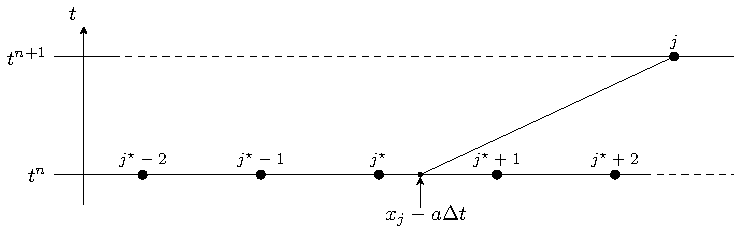
\includegraphics[width=0.9\textwidth]{\localPath/figures/semilag.pdf}
  \caption{Méthode des caractéristiques pour une méthode semi-lagrangienne avec une vitesse de transport $a>0$, et $d=2$.}
  \label{fig:intro:semilag}
\end{figure}


% --------------------------------------------------------------------
\subsection{Méthode pseudo-spectrale}
% --------------------------------------------------------------------

Une autre méthode souvent utilisée pour la résolution d'équations aux dérivées partielles est la méthode pseudo-spectrale qui consiste à approcher les opérateurs différentiels dans l'espace de Fourier à l'aide de transformées de Fourier. Cette méthode permet de transformer une équation aux dérivées partielles en un système d'équations différentielles ordinaires en transformant par exemple une dérivée dans l'espace réel en un produit dans l'espace de Fourier. Nous considèrerons ici la transformée de Fourier discrète, cela consiste à réécrire notre fonction $u$, $L$-périodique et de classe $C^1$, sous la forme :
$$
  u(x) = \sum_{\kappa=-\infty}^{+\infty} \hat{u}_\kappa e^{i\frac{2\pi \kappa}{L}x},
$$
où les coefficients de Fourier $\hat{u}_\kappa$ sont définis par :
$$
  \hat{u}_\kappa = \frac{1}{L}\int_0^L u(x)e^{-i\frac{2\pi \kappa}{L}x}\dd{x}.
$$

En n'ayant la connaissance de la fonction $u$ qu'en des points $x_j = j\frac{L}{N}$, $j=0,\dots,N-1$ de la grille, il est possible d'approcher les coefficient de Fourier par une somme discrète :
$$
  \hat{u}_\kappa \approx \frac{1}{N-1}\sum_{j=0}^N u(x_j) e^{=i\frac{2\pi j}{N}\kappa}.
$$

Transformer une dérivée en un produit nous sera utile au long de ce travail dans deux contextes, un premier linéaire :
$$
  \partial_t u + a\partial_x u = 0,\qquad u(t=0,x)=u_0(x)
$$
devenant après une transformée de Fourier : $\partial_t \hat{u}_\kappa + ai\kappa \hat{u}_\kappa = 0$ et pouvant se résoudre exactement en temps : $\hat{u}_\kappa(t) = \exp(-ia\kappa t)\hat{u}_\kappa(0)$. Cela correspond à la partie linéaire d'une méthode de Lawson~\ref{ssec:0:lawson}. L'autre cas d'utilisation sera pour un terme non-linéaire de la forme :
$$
  \partial_t u + \partial_xf(u) = 0,\qquad u(t=0,x)=u_0(x)
$$
devenant alors après une transformée de Fourier : $\partial_t\hat{u}_\kappa + i\kappa\widehat{\left(f(u)\right)}_\kappa = 0$. Ce terme n'ayant pas de solution explicite il sera résolu numériquement pas une méthode Runge-Kutta, correspondant au terme non-linéaire d'une méthode de Lawson.

Nous utiliserons l'algorithme de transformée de Fourier rapide (\emph{fast Fourier transform} ou FFT) pour effectuer numériquement cette opération, dont une implémentation est proposée dans~\cite{Saramito:2013}. Cet algorithme possède une complexité en temps de $\order{N\log N}$, où $N$ est le nombre de points de discrétisation en espace.

%% section 4
% !TEX root = ../../main.tex

\section{Résultats numériques}
\label{sec:3:num}

Dans cette section on s'intéresse à des résultats numériques pour la résolution du modèle VHL par les méthodes présentées précédemment. Conformément à~\cite{Holderied:2020}, nous considérons la condition initiale suivante :
$$
  f_h(t=0,z,\vb{v}) = \frac{\rho_h}{(2\pi)^{3/2}\bar{v}_{\|}\bar{v}_\perp^2}\exp( - \frac{v_z^2}{2\bar{v}_{\|}^2} - \frac{\left( v_x^2 + v_y^2 \right)^2}{2\bar{v}_\perp^2} )
$$
avec $z\in[0,\frac{2\pi}{k}]$, $k=2$, $\bar{v}_{\|}=0.2$, $\bar{v}_\perp=0.6$, $\rho_h=0.2$ et $B_x(t=0,z)=\epsilon\sin(kz)$. Les autres inconnues du système $(j_{c,x},j_{c,y},B_y,E_x,E_y)$ sont initialisées à zéro. Le domaine en vitesse est restreint à $\vb{v}\in[-3.6,3.6]\times[-3.6,3.6]\times[-2.4,2.4]$ et on note $N_z$, $N_{v_x}$, $N_{v_y}$, $N_{v_z}$ le nombre de points de discrétisation dans chaque direction. Dans chacune des simulations, on s'intéresse à l'évolution temporelle des énergies suivantes :
\begin{description}
  \item[Énergie magnétique : ] \begin{equation}\label{eq:3:nrj:me}\mathcal{H}_B(t) = \frac{1}{2}\int \left( B_x^2(t,z) + B_y^2(t,z) \right)\dd{z}\end{equation}
  \item[Énergie électrique : ] \begin{equation}\label{eq:3:nrj:ee}\mathcal{H}_E(t) = \frac{1}{2}\int \left( E_x^2(t,z) + E_y^2(t,z) \right)\dd{z}\end{equation}
  \item[Énergie cinétique des particules froides : ] \begin{equation}\label{eq:3:nrj:ce}\mathcal{H}_c(t) = \frac{1}{2\Omega_{pe}^2}\int \left( j_{c,x}^2(t,z) + j_{c,y}^2(t,z) \right)\dd{z}\end{equation}
  \item[Énergie cinétique des particules chaudes :  ] \begin{equation}\label{eq:3:nrj:he}\mathcal{H}_h(t) = \frac{1}{2}\iint |\vb{v}|^2 f_h(t,z,\vb{v}) \dd{\vb{v}}\dd{z}\end{equation}
\end{description}
dont la somme, l'énergie totale, est préservée au cours du temps :
$$
  \dv{\mathcal{H}}{t} = \dv{\mathcal{H}_B+\mathcal{H}_E+\mathcal{H}_c+\mathcal{H}_h}{t} = 0.
$$
Les diagnostics que nous regarderons pour vérifier la validité des résultats sont les différentes énergies au cours du temps, en vérifiant le taux d'instabilité donné par les relations de dispersion, présentées dans~\cite{Holderied:2020}. La comparaison entre les méthodes de résolution se fera à partir de la préservation de l'énergie totale $\mathcal{H}$, et de l'erreur relative produite par chacune des méthodes, nous comparerons également les temps de calcul.

%%%%%%%%%%%%%%%%%%%%%%%%%%%%%%%%%%%%%%%%%%%%%%%%%%%%%%%%%%%%%%%%%%%%%

\FloatBarrier
\subsection{Comparaison des solveurs à pas de temps constant}
% -------------------------------------------------------------------

Dans un premier temps nous considérons la méthode de \emph{splitting} et de Lawson avec un pas de temps constant, comme présenté dans la section~\ref{sec:3:scheme}. Nous présentons trois méthodes de \emph{splitting}, à savoir les méthodes de Lie, Strang et de Suzuki. La méthode de Suzuki ne sera présente qu'à titre d'illustration mais celle-ci n'est pas très intéressante dans un contexte multidimensionel, en effet ses résultats sont très similaires à la méthode de Strang, mais son temps de calcul représente 5 fois celui de cette méthode d'ordre 2. Dès que l'hamiltonien se subdivise en de nombreuses parties (7 dans notre cas), le nombre d'étapes requises pour obtenir de l'ordre élevé augmente drastiquement (même si certaines stratégies peuvent être utilisées pour éviter cela, comme présentées dans~\cite{Casas:2017}). La méthode de Strang nécessite à elle seule 15 étapes, ce qui représente $5\times15=75$ étapes par itération, ce qui est trop important pour que la méthode soit compétitive. Nous présenterons également deux méthodes de Lawson, la méthode LRK(3,3) et LRK(4,4) induites respectivement par la méthode RK(3,3) de Shu-Osher et la méthode RK(4,4) dite classique. Contrairement aux méthodes de \emph{splitting}, les méthodes de Lawson ne sont pas trop impactées par la montée en ordre dans le sens où le nombre d'étages nécessaire correspond, \emph{à peu près}, à l'ordre de la méthode. De plus, il existe une souplesse intrinsèque aux méthodes de Lawson qui réside dans le choix de la partie linéaire. Ce choix permet, par exemple, de se soustraire de certaines conditions de stabilités, sous contrainte du calcul de l'exponentielle de cette partie, problème contourné dans la section~\ref{s3:approx}. De plus le filtrage possible du terme $\vb{v}\times\vb{B}$ est intéressant dans les méthodes de Lawson car il permet de relaxer la condition de stabilité de la méthode. Un filtrage similaire serait envisageable dans les méthodes de \emph{splitting}, avec comme coût l'ajout de sous-étapes supplémentaires dans l'étape $\mathcal{H}_{f_h}$, étape déjà la plus coûteuse numériquement.

L'utilisation de schémas explicites introduit une condition de stabilité dans la résolution des équations de Maxwell, dans les deux approches (méthode de \emph{splitting} et de Lawson), présentée dans~\cite{Kormann:2021}. Il est également possible de se concentrer uniquement sur les inconnues $(B_x,B_y,E_x,E_y)$ pour déduire une condition de stabilité, comme vu dans la sous-section~\ref{ssec:3:cflMaxwell}. Le tableau~\ref{tab:CFL_maxwell} résume les différentes conditions de stabilité. Pour les méthodes de Lawson une condition de CFL supplémentaire provient de la discrétisation en vitesse, mais on remarque numériquement que cette dernière est moins contraignante que la condition provenant des équations de Maxwell. Nous verrons dans la section~\ref{s3:approx} comment s'affranchir de cette condition en intégrant les équations de Maxwell dans la partie linéaire de la méthode de Lawson.

\begin{table}[h]
  \centering
  \begin{tabular}{c|c}
    méthode         & condition de CFL          \\
    \hline
    Lie             & $(\sqrt{2}/\pi) \Delta z$ \\ 
    Strang          & $(2/\pi)\Delta z$         \\
    Lawson-RK(3, 3) & $(\sqrt{3}/\pi)\Delta z$  \\ 
    Lawson-RK(4, 4) & $(2\sqrt{2}/\pi) \Delta z$  
  \end{tabular}
  \caption{Condition de stabilité provenant des équations de Maxwell en utilisant différents intégrateurs.} 
  \label{tab:CFL_maxwell}
\end{table}

Nous traçons, sur la figure~\ref{fig:energies4d} l'évolution des énergies électrique, magnétique et l'énergie cinétique provenant des particules froides, définies précédemment, en échelle semi-log, pour différentes méthodes de \emph{splitting} (méthode de Lie, de Strang, et de Suzuki), et différentes méthodes de Lawson (LRK(3,3) et LRK(4,4), l'adjectif \emph{filtred} fait référence au filtrage mis en place dans la section~\ref{ssec:3:filtrage}). On choisit le maillage $27\times32\times32\times41$ et $\Delta t=0.05$ (ce qui assure la stabilité de toutes les méthodes présentées). On considère une faible perturbation $\epsilon = 10^{-5}$, pour assurer une longue phase linéaire (jusqu'au temps $t\approx 100$) tandis que la phase non-linéaire se développe jusqu'au temps final $t=200$. Dans la partie linéaire, il est possible de comparer les résultats numériques avec les solutions des relations de dispersion présentées dans~\cite{Holderied:2020}. Comme attendu, les trois énergies suivent une croissance exponentielle, avec le taux prédit par la théorie linéaire, ce qui se traduit par des transferts d'énergie des particules rapides (chaudes) vers l'énergie électro-magnétique et aux particules froides. Après la phase linéaire, les champs saturent en amplitude, ce qui marque l'effet des termes non-linéaires, la théorie linéaire n'est plus valide. On remarque que les deux classes de méthodes capturent efficacement les différents phénomènes en jeu dans la phase linéaire, avec une très bonne corrélation avec les taux d'instabilités calculés à l'aide de la théorie linéaire. De plus les différentes méthodes saturent à des niveaux d'énergie très similaires.

La figure~\ref{fig:energy_tot4d} représente l'erreur relative sur l'énergie totale, et permet d'étudier la conservation de celle-ci par les différentes méthodes. Bien que le maillage en espace soit très grossier ($\Delta z = \frac{2\pi}{27} \approx 0.23$) l'énergie totale est plutôt bien préservée : aux alentours de $8\%$ pour les deux méthodes de Lawson présentées, et autour de $5\%$ d'erreur pour les méthodes de Lie et de Strang. La méthode de Suzuki produit bien plus d'erreur (autour de $12\%$) très certainement à cause des multiples transformées de Fourier selon l'axe $z$ effectuées avec peu de points de discrétisation. Comme attendu, et observé dans le cas $1dx-1dv$, les méthodes basées sur un \emph{splitting} hamiltonien ont une bonne préservation de l'énergie totale, mais les qualités de leurs résultats, surtout observable avec la méthode de Suzuki, suggère la nécessité de raffiner le maillage. Il est à souligner que le coût numérique de la méthode de Strang, est environ deux fois plus important que celui de la méthode LRK(3,3).

\begin{figure}[h]
  \centering
  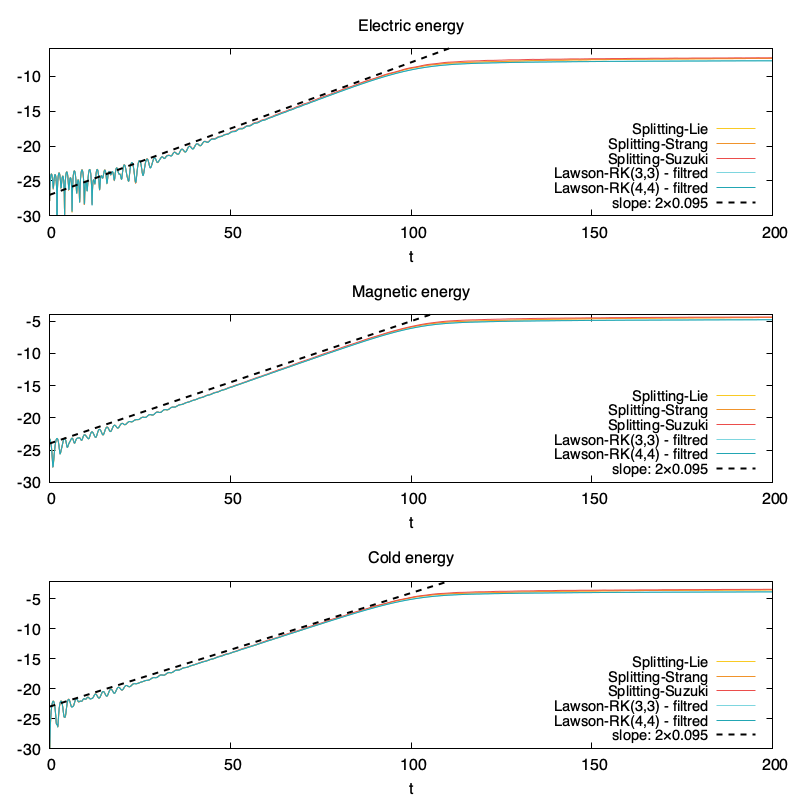
\includegraphics[width=0.9\textwidth]{\localPath/figures/energy_a_vmhl.png}
  \caption{Évolution de l'énergie électrique, magnétique et l'énergie cinétique des particules froides définies dans les équations~\ref{eq:3:nrj:me}-\ref{eq:3:nrj:ce}, en échelle semi-$\log$, pour les méthodes de \emph{splitting} de Lie, Strang et Suzuki, et pour les méthodes de Lawson LRK(3,3) et LRK(4,4). $\Delta t = 0.05, N_x=27, N_{v_x}=32, N_{v_y}=32, N_{v_z}=41$.}
  \label{fig:energies4d}
\end{figure}

\begin{figure}[h]
  \centering
  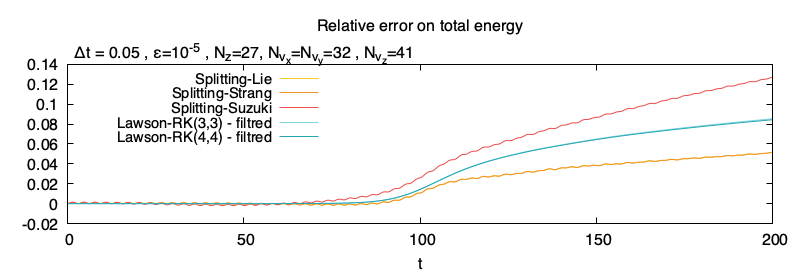
\includegraphics[width=0.9\textwidth]{\localPath/figures/H_a_vmhl.png}
  \caption{Évolution de l'erreur relative sur l'énergie totale, pour les méthodes de \emph{splitting} de Lie, Strang et Suzuki, et pour les méthodes de Lawson LRK(3,3) et LRK(4,4). $\Delta t = 0.05, N_x=27, N_{v_x}=32, N_{v_y}=32, N_{v_z}=41$.}
  \label{fig:energy_tot4d}
\end{figure}

On peut étudier l'importance du filtrage du terme $\vb{v}\times\vb{B}$ avec la figure~\ref{fig:compar_ee4d}, où l'on trace l'évolution de l'énergie électrique pour la méthode de Lawson LRK(3,3) avec ou sans le filtrage (voir l'algorithme~\ref{alg:modif} pour la différence algorithmique entre les deux méthodes) pour deux maillages différents de l'espace des phases ($15\times20\times20\times41$ à gauche et $15\times32\times32\times41$ à droite) avec un pas de temps $\Delta t = 0.1$. On peut observer l'impact sur les résultats du raffinement dans la direction $v_\perp$ sur la méthode non-filtrée, alors que sur la méthode filtrée on obtient un taux d'instabilité satisfaisant avec le maillage le plus grossier.

\begin{figure}[h]
  \centering
  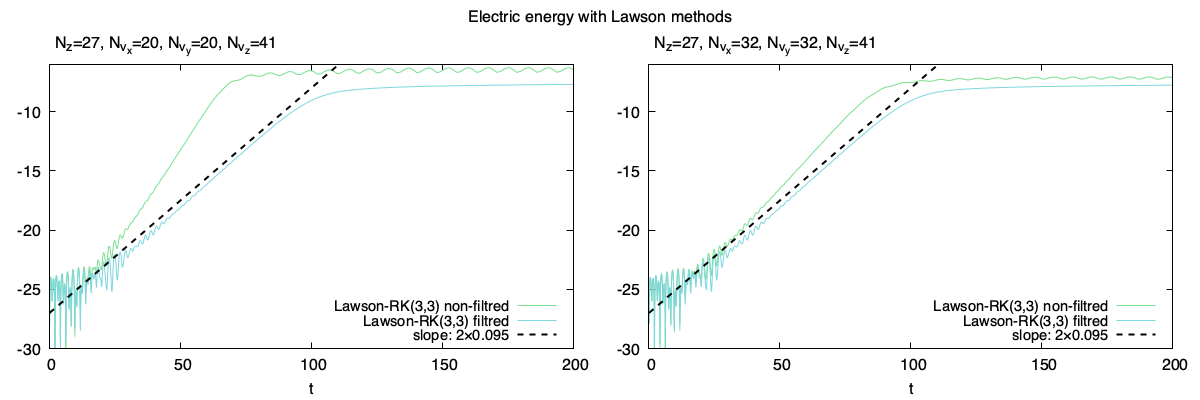
\includegraphics[width=0.9\textwidth]{\localPath/figures/ee_filtrage_vmhl.png}
  \caption{Évolution de l'énergie électrique pour les versions filtrées et non-filtrées de la méthode LRK(3,3) avec des maillages en vitesse différents. À gauche : $\Delta t = 0.05, N_x=27, N_{v_x}=20, N_{v_y}=20, N_{v_z}=41$. À droite : $\Delta t = 0.05, N_x=27, N_{v_x}=32, N_{v_y}=32, N_{v_z}=41$.}
  \label{fig:compar_ee4d}
\end{figure}


%%%%%%%%%%%%%%%%%%%%%%%%%%%%%%%%%%%%%%%%%%%%%%%%%%%%%%%%%%%%%%%%%%%%%

\FloatBarrier
\subsection{Étude à pas de temps adaptatif}
% -------------------------------------------------------------------
\label{ssec:3:dtn}

Le dernier test que nous souhaitons effectuer avec ces méthodes de résolution, est de considérer la méthode de Lawson à pas de temps adaptatif induite par le schéma DP4(3), comme dans la section \ref{ssec:dtadapt}. Pour que l'approche à pas de temps adaptatif soit intéressante dans notre cas il faut que :
\begin{enumerate}[label=(\roman*)]
  \item Les champs électromagnétiques soient suffisamment faibles dans la phase linéaire pour pouvoir prendre des grands pas de temps,\label{list:i}
  \item La condition de stabilité provenant des équations de Maxwell ne soit pas trop restrictive,\label{list:ii}
  \item Dans la phase non-linéaire, l'estimateur d'erreur nous assure la stabilité.\label{list:iii}
\end{enumerate}
En pratique, à cause de la discrétisation en espace la condition~\ref{list:ii} n'est pas satisfaite. Pour la suite nous considérons les paramètres numériques suivant : $N_z=27$, $N_{v_x}=32$, $N_{v_y}=32$, $N_{v_z}=41$, $tol=6\times10^{-5}$ et le pas de temps calculé par :
$$
  \Delta t_0 = \frac{C}{2}\Delta z,\quad \Delta t_{n+1} = \min\left( \max\left( \sqrt[p]{\frac{tol}{L_{[p]}^{n+1}}}\Delta t_n ,\frac{C}{2}\Delta z \right) , 3C\Delta z \right), n\geq 0
$$
où $L_{[p]}^{n+1}$ est l'erreur locale calculée par~\ref{eq:Lerror}, et $C$ est donné par le tableau~\ref{tab:CFL_maxwell}. La figure~\ref{fig:energieselecdp43} montre l'énergie électrique en échelle semi-log. Comme pour les méthodes présentées dans la section~\ref{ssec:2:dtn} les résultats sur les énergies sont très similaires, on capture le bon taux d'instabilité. On regarde sur la figure~\ref{fig:dtanderrordp43} deux diagnostics sur la méthode LDP4(3). Tout d'abord l'évolution de la taille des pas de temps au cours du temps (figure du haut). La simulation avec LDP4(3) est initialisée avec un pas de temps $\Delta t_0=0.05\approx\frac{1}{2}\frac{2\sqrt{2}}{N_z}$, les 3 itérations suivantes sont effectuées avec le pas de temps $\Delta t_n=3\frac{2\sqrt{2}}{N_z}$ qui est la borne supérieure que peut prendre le pas de temps $\Delta t_n$ (pour minimiser l'erreur générée en début de simulation, les champs électromagnétiques étant très faibles, l'estimateur d'erreur $L_{[p]}^{n+1}$ permet de prendre des pas de temps supérieurs à $1$) ; les autres itérations sont effectuées avec un pas de temps très proche de la condition de stabilité provenant des équations de Maxwell. Dans la phase linéaire, jusqu'au temps $t\approx 100$, la condition~\ref{list:ii} n'est pas satisfaite, la résolution des équations de Maxwell impose une condition CFL forte. Dans la phase non-linéaire, du temps $t\approx100$ jusqu'au temps final $t=200$, la condition de stabilité induite par le transport dans les directions $(v_x,v_y,v_z)$ n'est pas trop contraignante, ce qui permet de satisfaire la condition~\ref{list:iii} avec une contrainte pas trop forte. On remarque tout de même que la méthode LDP4(3) permet de prendre des pas de temps légèrement supérieurs à cette condition de stabilité, en effet $16\%$ des itérations réussies ont un pas de temps $\Delta t_n$ supérieur à la condition de stabilité $\frac{2\sqrt{2}}{N_z}$. La deuxième partie de la figure~\ref{fig:dtanderrordp43}, celle du bas, présente l'erreur locale au cours du temps, sont tracées également, par des carrés, les itérations rejetées. Contrairement au cas $1dx-1dv$, où le surcoût engendré par les itérations rejetées était négligeable, ici, seulement $71\%$ des itérations sont acceptées par le critère d'erreur.

\begin{figure}[h]
  \centering
  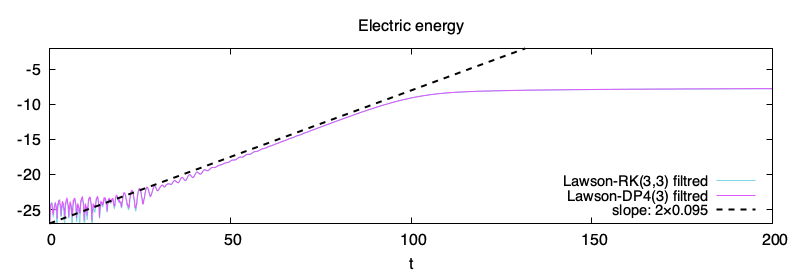
\includegraphics[width=0.77\textwidth]{\localPath/figures/energy_dp43_vmhl.png}
  \caption{Évolution de l'énergie électrique définie dans~\eqref{eq:3:nrj:ee}, en échelle semi-$\log$ pour les méthodes LRK(3,3) ($\Delta t = 0.05$) et LDP4(3). $N_x=27, N_{v_x}=32, N_{v_y}=32, N_{v_z}=41$.}
  \label{fig:energieselecdp43}
\end{figure}

\begin{figure}[h]
  \centering
  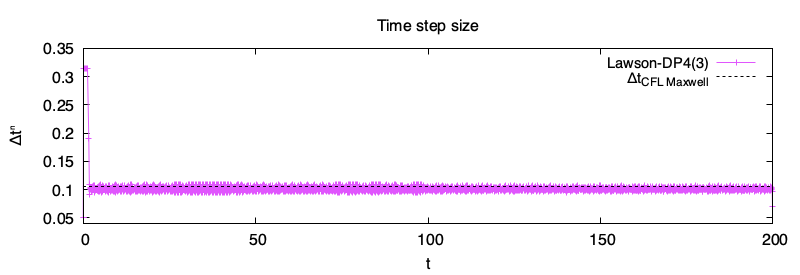
\includegraphics[width=0.77\textwidth]{\localPath/figures/dt_size_vmhl.png}
  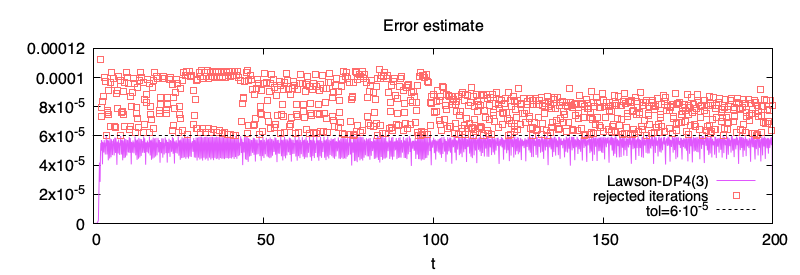
\includegraphics[width=0.77\textwidth]{\localPath/figures/L_vmhl.png}
  \caption{Évolution au cours du temps de la taille du pas du temps (haut) et de l'erreur locale (bas) pour la méthode de Lawson LDP4(3). $N_x=27, N_{v_x}=32, N_{v_y}=32, N_{v_z}=41$.}
  \label{fig:dtanderrordp43}
\end{figure}


%% section 5
% !TEX root = ../../main.tex

\section{Approximation de la partie linéaire}
\label{s3:approx}

L'obtention, à l'aide d'un logiciel de calcul formel, de l'exponentielle de la partie linéaire n'est pas toujours envisageable. Il est possible de recourir à une méthode d'approximation pour obtenir une formulation formelle de celle-ci qui sera possible d'utiliser pour l'écriture du code de simulation. On s'intéressera dans cette section à la partie linéaire $L$ définie par :
$$
  L = \begin{pmatrix}
    0   & -B_0 & 0          &  0          &  \Omega_{pe}^2 & 0             & 0 \\
    B_0 &  0   & 0          &  0          &  0             & \Omega_{pe}^2 & 0 \\
    0   &  0   & 0          &  0          &  0             & \partial_z    & 0 \\
    0   &  0   & 0          &  0          & -\partial_z    & 0             & 0 \\
   -1   &  0   & 0          & -\partial_z &  0             & 0             & 0 \\
    0   & -1   & \partial_z &  0          &  0             & 0             & 0 \\
    0   &  0   & 0          &  0          &  0             & 0             & -v_z\partial_z \\
  \end{pmatrix}
$$
Cette matrice est de la forme :
$$
  L = \begin{pmatrix}
    A & 0 \\
    0 & -v_z\partial_z
  \end{pmatrix}
$$
matrice diagonale par blocs, dont seul le bloc $A$ pose problème pour calculer formellement l'exponentielle. Ainsi on s'intéressera surtout à la sous-matrice $A$ obtenue après une transformée de Fourier en $z$ du système :
$$
  A = \begin{pmatrix}
    0 & -1 & 0  &  0  &  4  & 0  \\
    1 &  0 & 0  &  0  &  0  & 4  \\
    0 &  0 & 0  &  0  &  0  & ik \\
    0 &  0 & 0  &  0  & -ik & 0  \\
   -1 &  0 & 0  & -ik &  0  & 0  \\
    0 & -1 & ik &  0  &  0  & 0  \\
  \end{pmatrix}
$$
Par abus de notation, nous noterons $A_0$, la matrice $A$ pour $k=0$, ce qui revient à une partie linéaire sans les équations de Maxwell, ceci sera utile lors de la comparaison des résultats entre les méthodes.


\subsection{Troncature de la série de Taylor}
%--------------------------------------------------------------------

On peut définir $e^{tA}$ par la série de Taylor :
$$
  e^{tA} = \sum_{n=0}^\infty \frac{t^nA^n}{n!}.
$$
Une troncature d'ordre suffisamment élevé permet d'obtenir une approximation de l'exponentielle $e^{tA}$ à un ordre plus élevé que la méthode LRK($s$,$n$) où elle sera utilisé garanti que l'erreur de troncature reste inférieur à $n$, l'ordre de la méthode en temps. On définit la troncature de la série de Taylor à l'ordre $p$ par :
$$
  T_p(A) = \sum_{k=0}^p \frac{A^k}{k!}
$$

On sait que les valeurs propres de $A$ sont imaginaires pures, cela signifie que les valeurs propres de $e^{A}$ sont de norme 1.

\begin{figure}
  \begin{subfigure}{.5\textwidth}
    \centering
    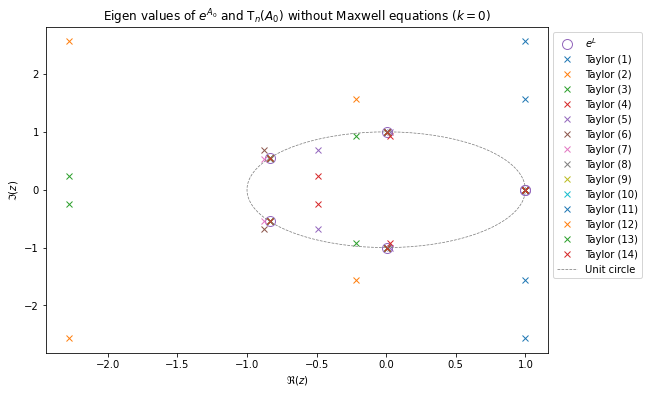
\includegraphics[width=\textwidth]{\localPath/figures/approx_evA0T5.png}
    \caption{Les valeurs propres de $e^{A_0}$ et de $T_5(A_0)$}
  \end{subfigure}
  \begin{subfigure}{.5\textwidth}
    \centering
    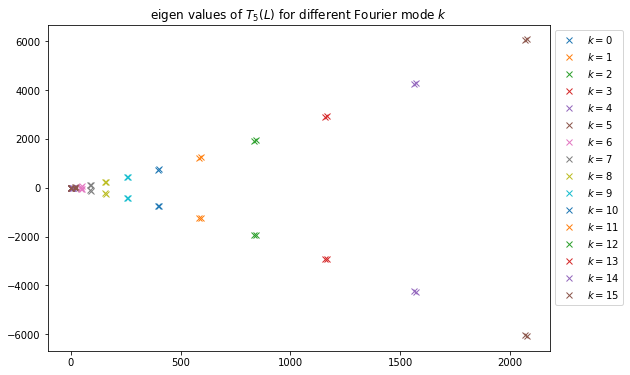
\includegraphics[width=\textwidth]{\localPath/figures/approx_evAkT5.png}
    \caption{Les valeurs propres de $e^{A}$ et de $T_5(A)$ pour différentes valeurs de $k\in[\![0,15]\!]$, par symétrie on obtient aussi celles pour $k<0$}
  \end{subfigure}
  \caption{Valeurs propres de $e^{A}$ et de $T_5(A)$ pour $k=0$ (sans les équations de Maxwell) à gauche, et pour différentes valeurs de $k\in[\![0,15]\!]$ à droite.}
\end{figure}

\Josselin{Je ne sais pas trop quoi dire sur les figures, donc je vais les mettre là un peu en vrac, on pourra discuter de leur intérêt plus tard, mais je pense qu'un petit calcul juste dire que les valeurs propres de $T_p(A)$ ne sont pas de module 1 serait plus intéressant.}

\begin{figure}
  \begin{subfigure}{.5\textwidth}
    \centering
    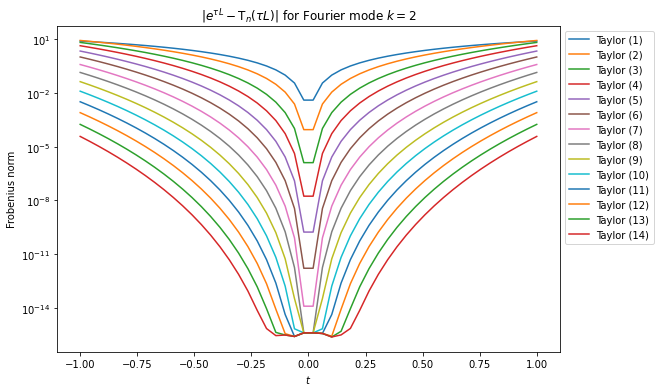
\includegraphics[width=\textwidth]{\localPath/figures/approx_errortA2T.png}
    \caption{L'erreur absolue locale $\|e^{tA}-T_p(tA)\|$ pour le mode de Fourier $k=2$}
  \end{subfigure}
  \begin{subfigure}{.5\textwidth}
    \centering
    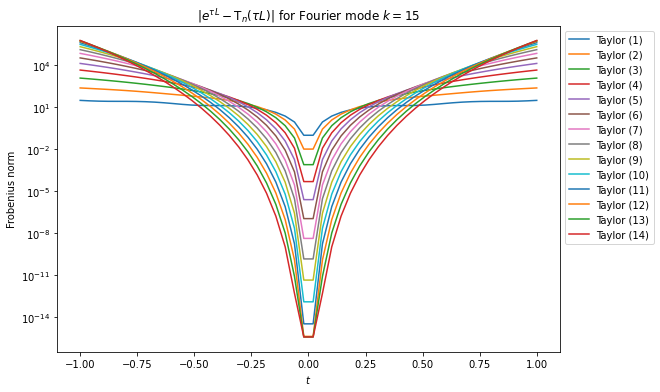
\includegraphics[width=\textwidth]{\localPath/figures/approx_errortA15T.png}
    \caption{L'erreur absolue locale $\|e^{tA}-T_p(tA)\|$ pour le mode de Fourier $k=15$}
  \end{subfigure}
  \caption{Erreur absolue locale $\|e^{tA}-T_p(tA)\|$ pour deux modes de Fourier $k=2$ à gauche et $k=15$ à droite.}
\end{figure}

\begin{figure}
  \centering
  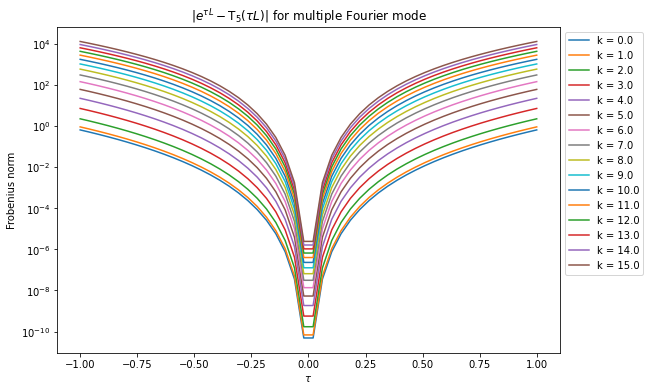
\includegraphics[width=0.75\textwidth]{\localPath/figures/approx_errortAkT5.png}
  \caption{L'erreur absolue locale $\|e^{tA}-T_5(tA)\|$ pour différents mode de Fourier}
\end{figure}

\subsection{Approximant de Padé}
%--------------------------------------------------------------------

Pour approcher une fonction, au lieu d'utiliser un polynôme comme dans le cadre des séries des développement limités, il est possible de construire une fraction rationnelle. L'approximant de Padé de la fonction exponentielle est la meilleure approximation de la fonction exponentielle par une fraction rationnelle et est définie par :
$$
  \begin{aligned}
    h_{p,q}(x) &= \sum_{i=0}^p \frac{\frac{p!}{(p-i)!}}{\frac{(p+q)!}{(p+q-i)!}}\frac{x^i}{i!} \\
    k_{p,q}(x) &= \sum_{j=0}^q (-1)^j \frac{\frac{q!}{(q-j)!}}{\frac{(p+q)!}{(p+q-j)!}} \frac{x^j}{j!}
  \end{aligned}
$$

$$
  p_{p,q}(x) = \frac{h_{p,q}(x)}{k_{p,q}(x)} \approx e^x
$$

Pour utiliser cet approximant de Padé, qui est une fraction rationnelle, avec des matrices il faut utiliser la définition suivante :

$$
  e^M \approx \textrm{P}_{p,q}(M) = h_{p,q}(M)\cdot\left(k_{p,q}(M)\right)^{-1}
$$

On effectue la même étude qu'avec une troncature de la série de Taylor. On regarde donc dans un premier temps sur la figure~\ref{fig:evAP22} les valeurs propres dans le cas $k=0$ et pour différentes valeurs de $k$.

\begin{figure}
  \begin{subfigure}{.5\textwidth}
    \centering
    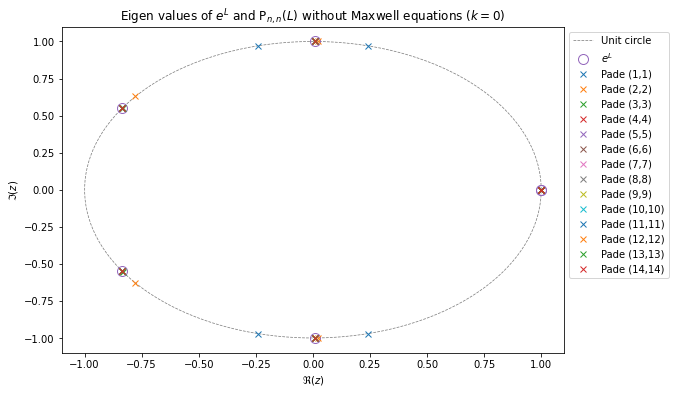
\includegraphics[width=\textwidth]{\localPath/figures/approx_evA0P.png}
    \caption{Les valeurs propres de $e^{A_0}$ et de $P_{n,n}(A_0)$}
  \end{subfigure}
  \begin{subfigure}{.5\textwidth}
    \centering
    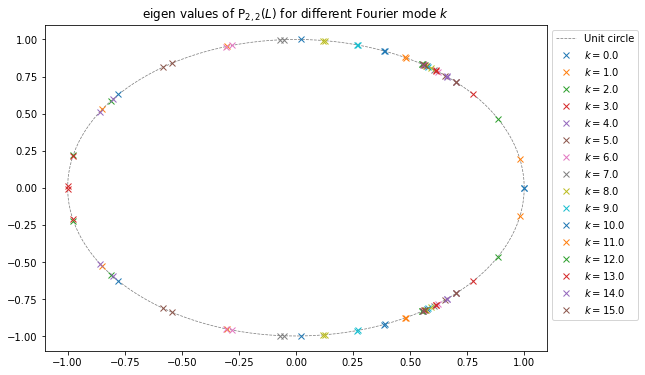
\includegraphics[width=\textwidth]{\localPath/figures/approx_evAkP22.png}
    \caption{Les valeurs propres de $e^{A}$ et de $P_{2,2}(A)$ pour différentes valeurs de $k\in[\![0,15]\!]$, par symétrie on obtient aussi celles pour $k<0$}
  \end{subfigure}
  \caption{Valeurs propres de $e^{A}$ et de $P_{n,n}(A)$ pour $k=0$ (sans les équations de Maxwell) à gauche, et pour différentes valeurs de $k\in[\![0,15]\!]$ à droite.}
  \label{fig:evAP22}
\end{figure}

\begin{figure}
  \begin{subfigure}{.5\textwidth}
    \centering
    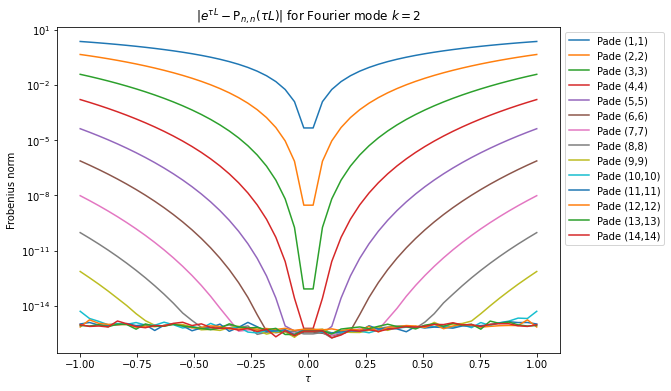
\includegraphics[width=\textwidth]{\localPath/figures/approx_errortA2P.png}
    \caption{L'erreur absolue locale $\|e^{tA}-T_p(tA)\|$ pour le mode de Fourier $k=2$}
  \end{subfigure}
  \begin{subfigure}{.5\textwidth}
    \centering
    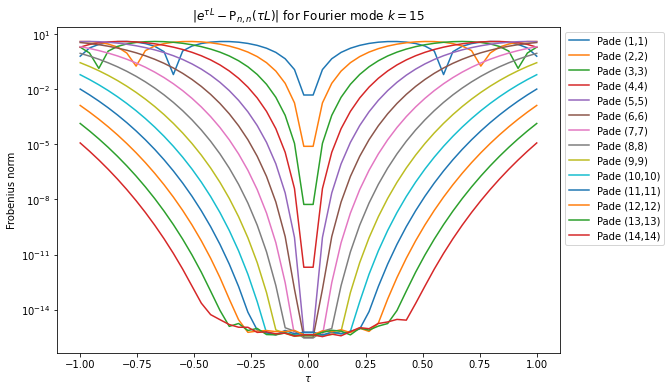
\includegraphics[width=\textwidth]{\localPath/figures/approx_errortA15P.png}
    \caption{L'erreur absolue locale $\|e^{tA}-T_p(tA)\|$ pour le mode de Fourier $k=15$}
  \end{subfigure}
  \caption{Erreur absolue locale $\|e^{tA}-T_p(tA)\|$ pour deux modes de Fourier $k=2$ à gauche et $k=15$ à droite.}
\end{figure}

\begin{figure}
  \centering
  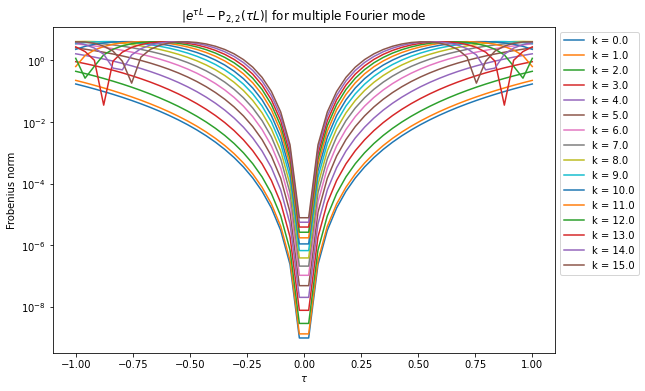
\includegraphics[width=0.75\textwidth]{\localPath/figures/approx_errortAkP22.png}
  \caption{L'erreur absolue locale $\|e^{tA}-T_5(tA)\|$ pour différents mode de Fourier}
\end{figure}



%% section 6
% !TEX root = ../../main.tex

\section{Résultats numériques des schémas de Lawson approchés}

\subsection{Comparaison des troncatures à pas de temps constant}

\subsection{Étude à pas de temps adaptatif}

\begin{otherlanguage}{english}
Acknowledgment: Experiments presented in this section were carried out using the PlaFRIM experimental testbed, supported by Inria, CNRS (LABRI and IMB), Université de Bordeaux, Bordeaux INP and Conseil Régional d’Aquitaine (see \url{https://www.plafrim.fr/}).
\end{otherlanguage}

%% section 7
% !TEX root = ../../main.tex

\section{Optimisations et performances}
\label{s:3:info}

Cette section s'intéresse aux aspects techniques de l'implémentation des schémas présentés dans la section~\ref{sec:3:scheme}. Il sera tout d'abord question de méthode de génération de code, utilisée uniquement dans le cadre de la méthode de Lawson, puis nous discuterons des performances et des choix d'implémentation effectués.

\subsection{Génération automatique de code}
\label{ssec:3:codegen}

La simulation d'un système à 7 inconnues, dont 1 inconnue à 4 dimensions, avec une méthode de type Lawson-Runge-Kutta (LRK) d'ordre élevé, nécessite de nombreuses lignes de code dont l'écriture peut s'avérer fastidieuse, entrainant de nombreuses possibilités de bugs informatiques. Une part importante de l'analyse ayant été réalisée à l'aide de la bibliothèque de calcul symbolique \Python{} : \sympy, il a été décidé de poursuivre son utilisation pour aider à l'écriture du code de simulation. Dans un premier temps cet usage s'est limité à une aide à l'écriture en générant chacune des 7 expressions pour chaque variable, et ce à chaque étage de la méthode LRK (3 étages pour RK(3,3), jusqu'à 5 étages pour une méthode comme DP4(3)). Des outils de méta-programmation, développés en \Python{}, ont été utilisés pour obtenir une génération complète du code à partir d'un squelette de code \CC{} et de l'écriture mathématique du schéma LRK que l'utilisateur souhaite utiliser.

Les expressions \sympy{} sont gérées comme des arbres syntaxiques dont les feuilles sont des nombres ou des symboles. Ces derniers vont servir à représenter des variables \CC, il est donc nécessaire dans un premier temps de s'assurer que la conversion de ces symboles en chaînes de caractères assure des noms de variables valide en \CC. En effet il est fréquent d'utiliser des symboles s'exportant facilement en \LaTeX{}, or un tel symbole n'est pas utilisable de la sorte comme nom de variable ; par exemple $\Delta t$ s'exportera par défaut en chaîne de caractères en "\texttt{\textbackslash Delta\textbackslash\ t}". Les nœuds de l'arbre syntaxique sont des fonctions, il y a alors deux cas à distinguer. Soit il s'agit d'une fonction dont la représentation en \Python{} est la même qu'en \CC, auquel cas aucune opération particulière n'est nécessaire ; c'est le cas par exemple des opérations arithmétiques $+$, $-$, $\times$ et $\divisionsymbol$ qui sont représentées par les opérateurs binaires \texttt{+}, \texttt{-}, \texttt{*} et \texttt{/} en \Python{} et \CC{}. Soit il s'agit d'une fonction dont la représentation \Python{} et \CC{} diffère, auquel cas il est nécessaire de créer une fonction \sympy{} qui aura le même nom que la fonction \CC{} associée, et de substituer le nœud de l'arbre syntaxique par cette nouvelle fonction. La conversion en chaîne de caractère de l'arbre ainsi modifié sera une expression \CC{} valide. Il est possible d'améliorer l'expression \CC{} en faisant une évaluation numérique des nombres rationnels (et potentiellement aussi irrationnels) présents, pour limiter le nombre d'opérations dans l'expression finale. Ainsi l'expression \texttt{1/3} sera substituée par \texttt{0.333333333333333}, cela permet d'éviter des interprétations de fractions comme des divisions entières par le compilateur.

Pour chaque étage de la méthode LRK, il est ainsi possible d'obtenir une expression \CC{} valide par variable. L'étape supplémentaire est d'utiliser un moteur de \emph{template} pour insérer ces expressions dans un squelette de code qui s'adapte automatiquement au nombre d'étages de la méthode LRK, en initialisant et allouant les variables temporaires nécessaires. Ce travail est effectué par le moteur de \emph{template} Jinja2, qui est une bibliothèque \Python{} permettant d'ajouter des opérations logiques en plus d'une simple substitution de champs dans un squelette de code préexistant. Le squelette en pseudo-code d'un étage d'une méthode LRK est donné en exemple dans l'algorithme~\ref{alg:squeltte} dans la section~\ref{ssec:3:stage}.

\paragraph{Nota Bene :} La bibliothèque \sympy{} contient des fonctions permettant la génération de code en C ou Fortran, mais le fonctionnement de celles-ci s'adapte mal à une intégration dans une boucle d'un code déjà existant. De plus les fonctions ainsi générées ne fonctionnent pas avec un code contenant des \emph{template} \CC, pour changer éventuellement de type pour de possibles optimisations. Elles ne prennent en paramètre que des valeurs par copie ou par pointeur, ce qui limite leur usage avec des structures de données évoluées proposées par les librairies \CC. Il serait envisageable d'utiliser certains des mécanismes présents dans ces fonctions pour améliorer la génération de code proposé ci-dessus, en utilisant un parcours d'arbre syntaxique pour construire un \emph{Abstract Syntax Tree} (AST) permettant la génération dans n'importe quel langage d'une expression. Les fonctions \sympy{} de génération de code sont encore en phase de développement et ne disposent pas d'une documentation complète. Les outils mis en place au cours de cette thèse pallient certains problèmes de \sympy{}, mais ne sont adaptés qu'à ce contexte précis.

\subsection{Performances}

Nous souhaitons dans cette section présenter les choix techniques effectués pour garantir la performance de l'implémentation des schémas détaillés dans la section~\ref{sec:3:scheme}. Nous essayerons aussi de quantifier cette performance avec ou sans parallélisation.

\subsubsection{Structure de données}

Le choix a été fait, durant toute cette thèse, d'utiliser une méthode spectrale pour résoudre le transport en espace (direction $x$ ou $z$). Cela implique d'effectuer régulièrement des transformées de Fourier, ou des transformées inverses. Pour effectuer ces opérations efficacement il est nécessaire que cette mémoire soit contigüe, cela indique qu'il s'agit du dernier indice dans les tableaux manipulés en \CC. La méthode WENO5, utilisée en vitesse, nécessite le \emph{stencil} représenté sur la figure~\ref{fig:3:stencil}. Mais cette représentation est trompeuse, en effet les différents points représentés ne sont pas contigus en mémoire, et les points $f_{[k_x,k_y,k_z,i]}$ et $f_{[k_x+1,k_y,k_z,i]}$, par exemple, sont distants de $N_z\times N_{v_z} \times N_{v_y} + 1$ cases mémoires ; la mémoire étant d'abord contigüe en $z$, puis $v_z$, $v_y$ et enfin $v_x$. Ainsi l'accès aux cases mémoires de ce \emph{stencil} est coûteux, conclusion confirmée par une étude à l'aide d'outils de profilage de code telle que le module Massif de Valgrind.

\begin{figure}
  \centering
  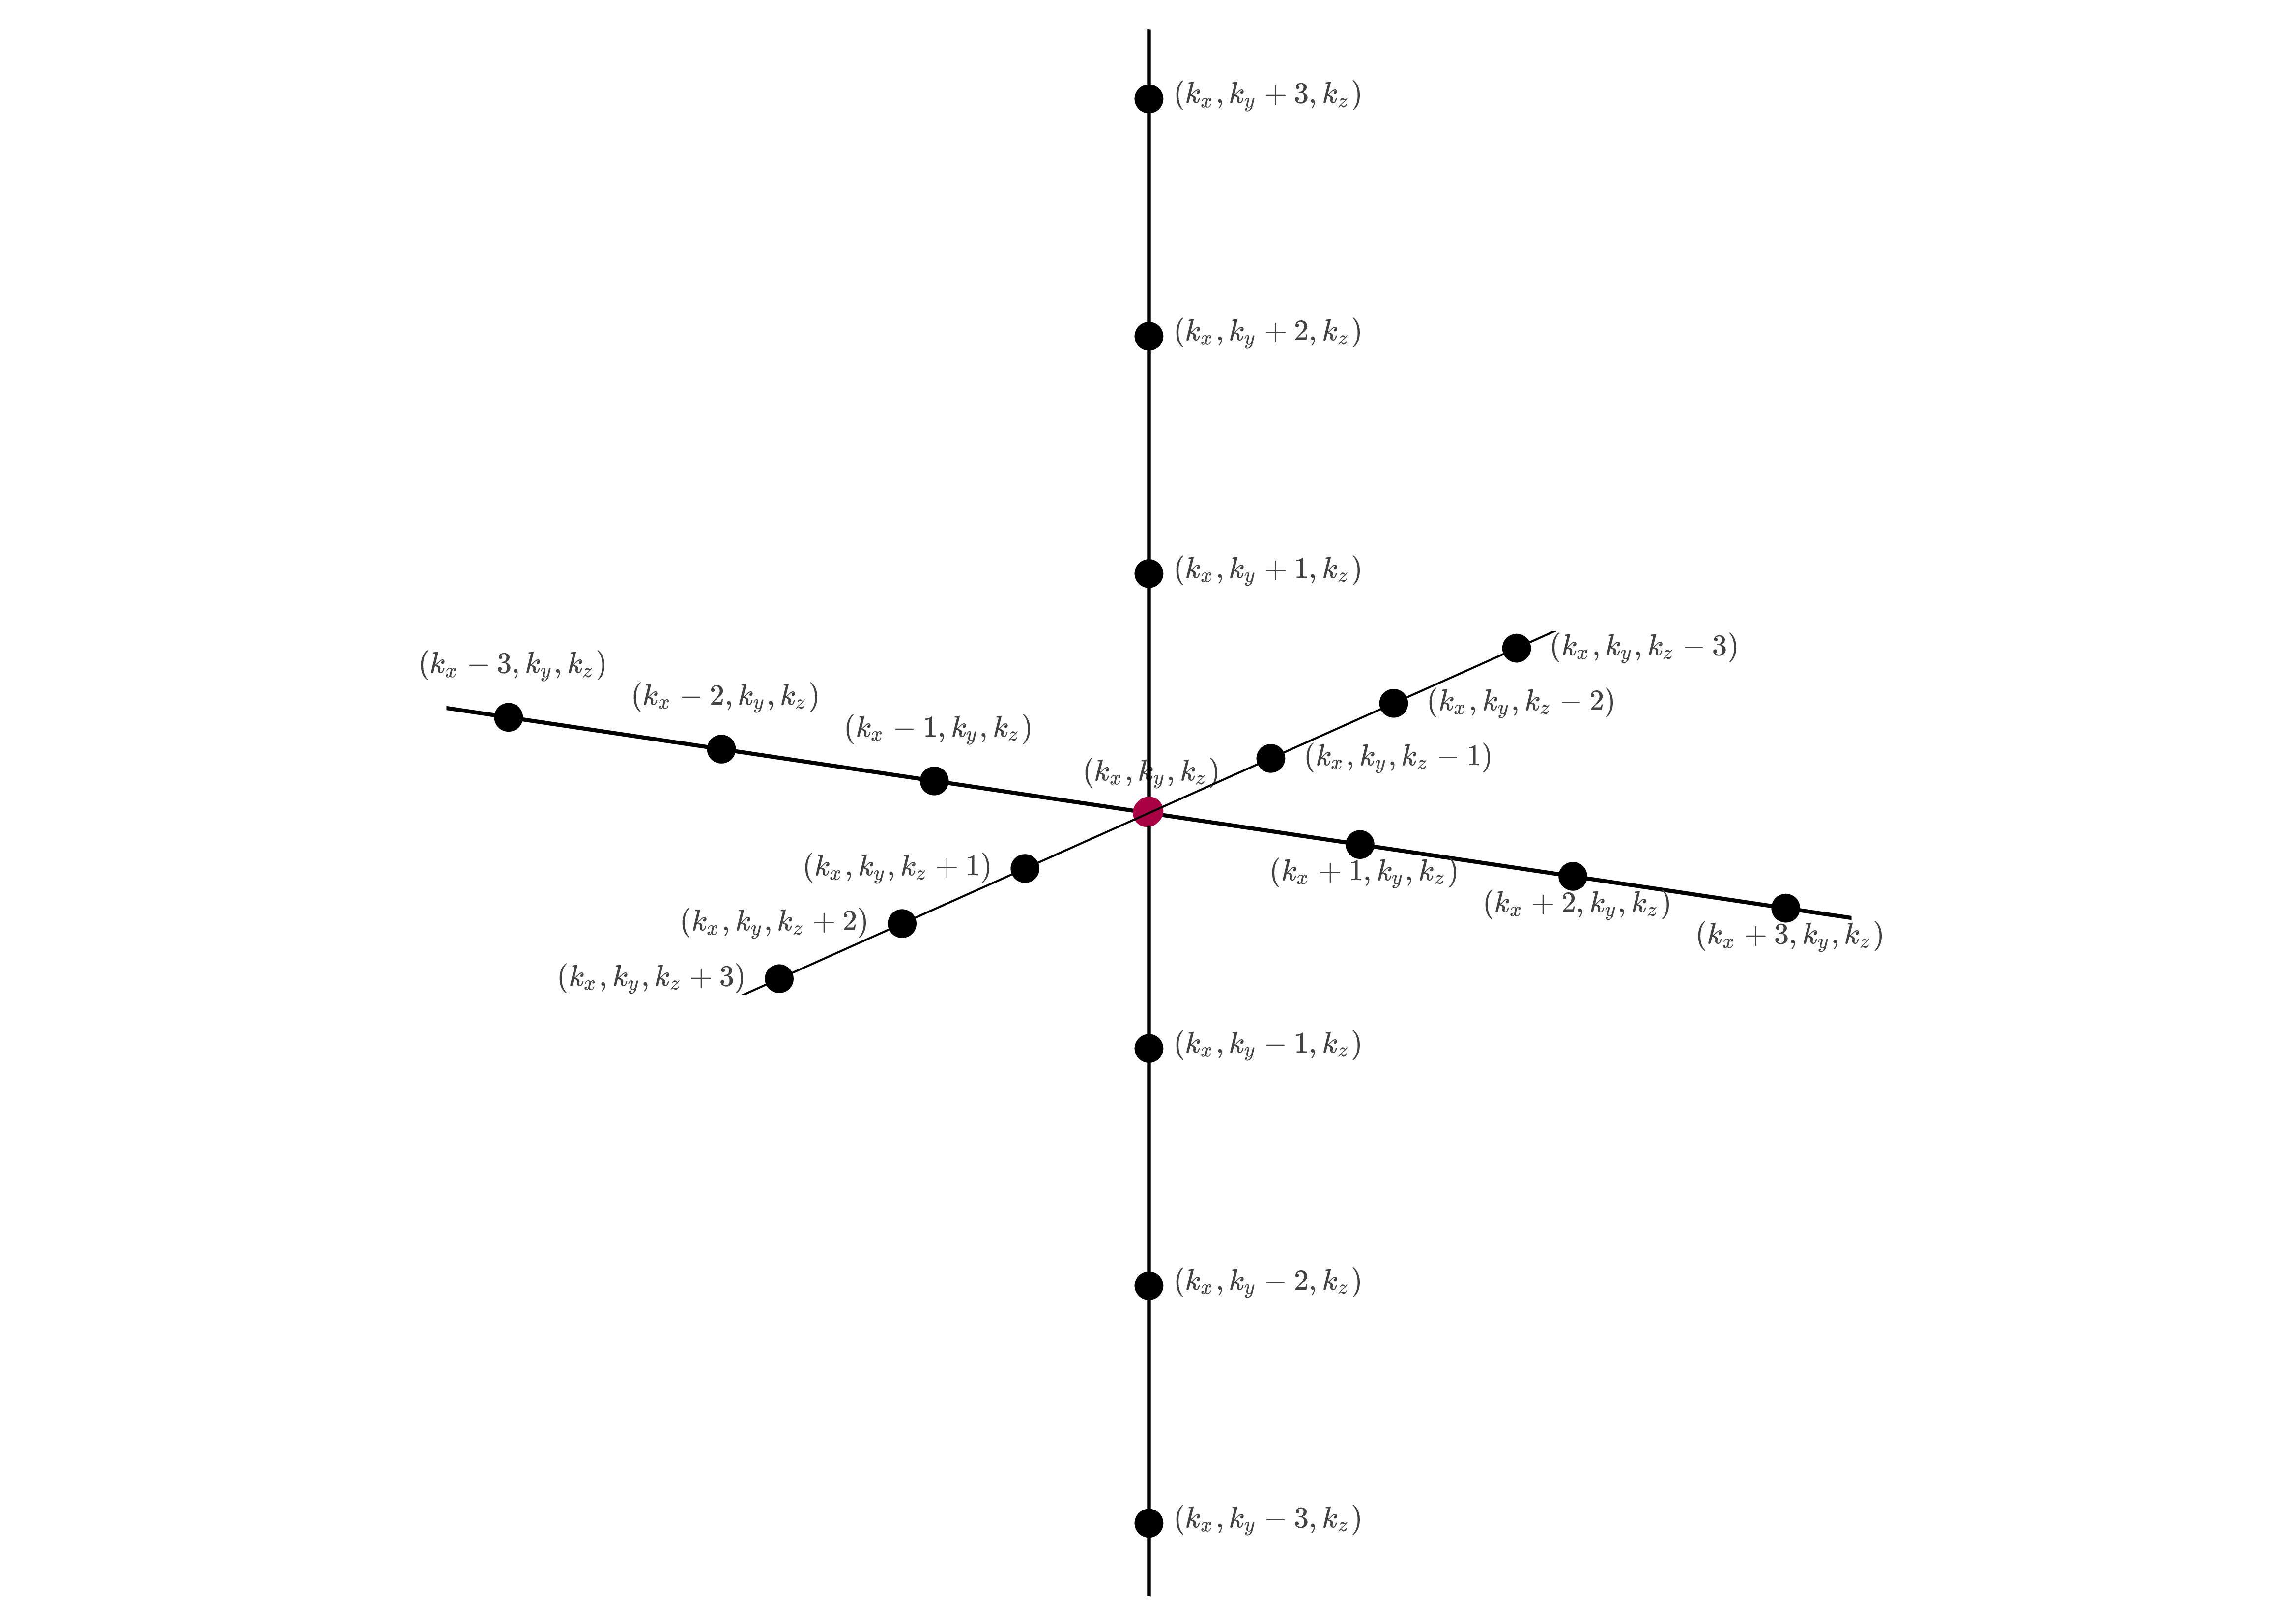
\includegraphics[width=0.75\textwidth]{\localPath/figures/stencil}
  \caption{Représentation à 3 dimensions du \emph{stencil}, centré sur le point $(k_x,k_y,k_z)$, de la méthode WENO5 utilisée pour résoudre le terme $(\vb{E}+\vb{v}\times\vb{B})\cdot\nabla_{\vb{v}}f$.}
  \label{fig:3:stencil}
\end{figure}

Cette structure est imposée par les différentes transformées de Fourier et transformées inverses effectuées dans la direction $z$ dans notre méthode de résolution, et est commune à la fois aux méthodes de \emph{splitting} et de Lawson. S'affranchir de transformées de Fourier (en restant dans l'espace complexe ou non) permettrait de structurer nos données selon une courbe d'Hilbert qui préserve bien la localité des données, rendant les accès mémoire aux données de ce \emph{stencil} moins coûteux.

\subsubsection{Performance séquentielle}

Le cadre multi-dimensionnel se prête moins au raffinement du maillage ou à de nombreux tests pour effectuer des mesures fines du pas de temps. Un test a tout de même été effectué avec toutes les simulations stables numériquement sur le maillage $N_z \times N_{v_x} \times N_{v_y} \times N_{v_z}=27\times32\times32\times41$ et avec un pas de temps constant $\Delta t=0.05$. Les temps de calcul sont présentés dans le tableau~\ref{tab:3:computing:time}, avec l'ajout de deux méthodes à pas de temps adaptatif (LDP4(3) et LDP4(3) - $P_{2,2}$) pour lesquelles le pas de temps $\Delta t=0.05$ n'est que le pas de temps initial. On remarque que l'approximation de l'exponentielle de la partie linéaire d'une méthode de Lawson, avec une série de Taylor ou un approximant de Padé, n'introduit pas de coût visible sur le temps de calcul. On remarque même un temps de calcul plus faible, qui peut être dû au coût de calcul de la fonction \texttt{std::exp}\footnote{La fonction \CC{} \texttt{std::exp} est la fonction exponentielle de la bibliothèque standard de \CC{}.}, utilisée dans les méthodes de Lawson exactes, par rapport à l'évaluation de fractions rationnelles nécessaires dans les méthodes de Lawson couplées à une série de Taylor ou un approximant de Padé.

\begin{table}[h]
  \centering
  \begin{tabular}{l|r}
    Méthode & temps de calcul \\
    \hline
    Méthode de Lie       &                $13\,\textrm{h}\ 25\,\textrm{min}\ 10\,\textrm{s}$ \\
    Méthode de Strang    &                $17\,\textrm{h}\ 09\,\textrm{min}\ 54\,\textrm{s}$ \\
    Méthode de Suzuki    & $3\,\textrm{j}\ 03\,\textrm{h}\ 05\,\textrm{min}\ 24\,\textrm{s}$ \\
    \hline
    LRK(3,3)             &                $11\,\textrm{h}\ 29\,\textrm{min}\ 09\,\textrm{s}$ \\
    LRK(3,3) - $T_4$     &                $10\,\textrm{h}\ 53\,\textrm{min}\ 40\,\textrm{s}$ \\
    LRK(3,3) - $P_{1,1}$ &                $10\,\textrm{h}\ 54\,\textrm{min}\ 11\,\textrm{s}$ \\
    LRK(3,3) - $P_{2,2}$ &                $10\,\textrm{h}\ 55\,\textrm{min}\ 26\,\textrm{s}$ \\
    \hline
    LRK(4,4)             &                $14\,\textrm{h}\ 06\,\textrm{min}\ 15\,\textrm{s}$ \\
    LRK(4,4) - $T_5$     &                $14\,\textrm{h}\ 00\,\textrm{min}\ 03\,\textrm{s}$ \\
    LRK(4,4) - $P_{2,2}$ &                $13\,\textrm{h}\ 59\,\textrm{min}\ 59\,\textrm{s}$ \\
    \hline
    LDP4(3)              &                $11\,\textrm{h}\ 44\,\textrm{min}\ 04\,\textrm{s}$ \\
    LDP4(3) - $P_{2,2}$  &                $04\,\textrm{h}\ 09\,\textrm{min}\ 44\,\textrm{s}$ \\
  \end{tabular}
  \caption{Temps de calcul pour les différentes simulations avec le maillage $N_z \times N_{v_x} \times N_{v_y} \times N_{v_z}=27\times32\times32\times41$ et le pas de temps $\Delta t = 0.05$ (pas de temps initial pour les deux simulations à pas de temps adaptatif).}
  \label{tab:3:computing:time}
\end{table}

Pour comparer également la qualité des résultats, en plus de leur vitesse d'obtention, nous traçons sur la figure~\ref{fig:3:H_time} l'erreur relative sur l'énergie totale pour différentes simulations. Pour la visibilité de la courbe, nous ne conservons ici que les simulations obtenues avec les méthodes de Strang, de Suzuki ainsi que les méthodes de Lawson LRK(4,4) et LDP4(3) couplées avec l'approximant de Padé $P_{2,2}$. On remarque que les méthodes géométriques (méthodes de Strang et de Suzuki), à cause du maillage trop grossier, n'ont pas le comportement attendu, c'est-à-dire une oscillation autour de zéro. La méthode de Strang, comme la méthode de Lie, donne une erreur relative bien plus intéressante ($5.1\%$) que la méthode de Suzuki ($12.1\%$). Les méthodes de Lawson donnent des erreurs relatives similaires, c'est-à-dire autour de $8.4\%$, c'est principalement le temps de calcul qui distingue ces différentes méthodes, et non la précision de leurs résultats, même pour les méthodes de Lawson d'ordre 3. L'impact faible de l'ordre de la méthode sur les résultats vient du maillage relativement grossier.

\begin{figure}
  \centering
  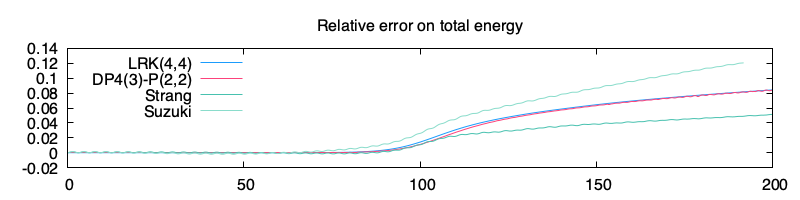
\includegraphics[width=\textwidth]{\localPath/figures/H_time.png}
  \caption{Comparaison de l'erreur relative au cours du temps pour différentes simulations : méthode de Strang, Suzuki, de Lawson $LRK(4,4)$ et la méthode de Lawson à pas de temps adaptatif couplée à un approximant de Padé $LDP4(3)-P_{2,2}$.}
  \label{fig:3:H_time}
\end{figure}

\subsubsection{Performance parallélisée}



%% section 8
% !TEX root = ../../main.tex

\section{Conclusion}
% -------------------------------------------------------------------

Au cours de ce chapitre nous avons pu étudier et confirmer numériquement la convergence du modèle cinétique $1dx-1dv$ vers le modèle hybride. Nous avons décrit deux méthodes de résolution du modèle hybride. La première méthode, méthode de \emph{splitting}, tirant parti de la structure hamiltonienne du système et assurant le bon comportement en temps long de certaines quantités (énergie, masse). La seconde méthode de résolution est basée sur une méthode de Lawson, et ne préserve aucune quantité particulière, mais permet une montée en ordre en temps pour un coup numérique plus faible. La comparaison des résultats s'est faite grâce à une étude fine des relations de dispersion, permettant de reconstruire le champ électrique et de déterminer le taux d'instabilité dans nos cas tests.

Un résultat supplémentaire que nous avons pu obtenir dans cette comparaison, est l'intérêt plus important de la méthode de pas de temps adaptatif basée sur la méthode de Lawson, permettant de profiter de toute la littérature sur les méthodes de type Runge-Kutta.

En perspective, il est possible d'étudier le modèle hybride, en tenant compte des termes non-linéaires dans la partie fluide. Dans un contexte plus perturbatif, il est possible que ceux-ci capturent mieux la solution du modèle cinétique, cadre où les hypothèse de linéarisation sont violées. 

Différentes perspectives sont en cours d'étude en ce qui concerne la résolution numérique. Il est envisageable d'augmenter la partie linéaire de l'équation de Vlasov-Ampère hybride linéarisé~\eqref{eq:vahl} en y intégrant le calcul du courant, en effet le système devient, après une transformée de Fourier en $x$, pour un mode de Fourier $\kappa$ :
$$
  \begin{cases}
    \partial_t\hat{f}_{h,\kappa} + i\kappa v\hat{f}_{h,\kappa} + \widehat{\left(E\partial_vf_h\right)}_\kappa = 0 \\
    \partial_t \hat{u}_{c,\kappa} = \hat{E}_\kappa \\
    \partial_t\hat{E}_\kappa = -\rho_c^{(0)}\hat{u}_{c,\kappa} -\int_\mathbb{R} v\hat{f}_{h,\kappa}\dd{v}.
  \end{cases}
$$
En discrétisant en $v$ le problème, et en calculant le courant induit par les particules chaudes $j_h$ à l'aide de la méthode des rectangles :
$$
  \int_\mathbb{R} v\hat{f}_{h,\kappa}\dd{v} = \hat{j}_h \approx \sum_{j=1}^{N_v} v_j\hat{f}_j\Delta v
$$
avec $v_j = -v_{\text{max}}+ j\Delta v$, il est possible de réécrire le problème comme :
$$
  \partial_t \begin{pmatrix}
    \hat{f}_{h,\kappa,1} \\
    \vdots \\
    \hat{f}_{h,\kappa,N_v} \\
    \hat{u}_{c,\kappa} \\
    \hat{E}_\kappa
  \end{pmatrix}
  =
  \begin{pmatrix}
    \mqty{
      \mqty{
        \mqty{\dmat{-i\kappa v_1,\ddots,-i\kappa v_{N_v}}} \\
        \mqty{0            &\cdots& 0               \\
              -v_1\Delta v &\cdots& -v_{N_v}\Delta v }
      }
      &
      \mqty{
        0             & 0      \\
        \vdots        & \vdots \\
        0             & 0      \\
        0             & 1      \\
        -\rho_c^{(0)} & 0
      }
    }
  \end{pmatrix}
  \begin{pmatrix}
    \hat{f}_{\kappa,1} \\
    \vdots \\
    \hat{f}_{\kappa,N_v} \\
    \hat{u}_{c,\kappa} \\
    \hat{E}_\kappa
  \end{pmatrix}
  +
  \begin{pmatrix}
    -\widehat{(E\partial_vf)}_{\kappa,1} \\
    \vdots \\
    -\widehat{(E\partial_vf)}_{\kappa,N_v} \\
    0 \\
    0
  \end{pmatrix}.
$$
Ceci s'applique également au modèle de Vlasov-Ampère~\eqref{eq:vlasov}-\eqref{eq:ampere}. Cette stratégie permet de garantir que l'équation de Poisson sous-jacente est satisfaite. De plus les contributions des estimateurs d'erreur $L_{u_c}$ et $L_E$ passent sous l'erreur machine car mettant en jeu que des variables résolues dans la partie linéaire (et donc exacte), dans le cadre d'une méthode à pas de temps adaptatif, comme présentée sur la figure~\ref{fig:compare:error:LucEfh}.

La résolution de ce problème avec une méthode de Lawson, permet d'envisager l'utilisation de méthodes de Lawson semi-implicites, permettant de lever des conditions de stabilité en $v$. Pour cela il est possible de construire des méthodes de Lawson induites par une méthode DIRK (\emph{Diagonally Implicit Runge-Kutta}), famille de méthodes présentée dans~\cite{Alexander:1976}, une autre stratégie est l'utilisation de méthodes IMEX à partir d'une méthode DIRK comme dans~\cite{Cho:2021}. Rendre implicite des termes, plus particulièrement ceux résolus par une méthode non-linéaire comme WENO est un problème compliqué. Une proposition d'inversion de WENO est présenté dans~\cite{Gottlieb:2006}, avec la méthode iWENO (\emph{implicit WENO}), entraînant des oscillations. Il est également possible de s'appuyer sur les travaux présentés dans~\cite{Boscarino:2019} où est utilisé une méthode de WENO dans un contexte de méthode IMEX en temps. Si on accepte le coût numérique engendré par la méthode implicite il peut être intéressant de s'intéresser aux méthodes AVF (\emph{Averaged Vector Field}) qui permettent de conserver l'énergie totale. Dans~\cite{Mei:2021}, les auteurs combinent le schéma exponentiel et la méthode AVF dans un contexte d'équation différentielles ordinaires ; la généralisation au cas des équations aux dérivées partielles n'est pas triviale mais intéressante.

Nous allons voir dans le chapitre suivant comment s'effectue la montée en dimension du modèle et de sa résolution numérique. Celle-ci engendre de nombreuses modifications, à la fois sur le nombre d'étapes de la méthode de \emph{splitting}, et sur la discrétisation envisageable pour une méthode de Lawson en $(x,\vb{v})$. Les conclusions obtenues, à propos de la performance de certaines méthodes, seront différentes.


